%%%%%%%%%%%%%%%%%%%%%%%%%%%%%%%%%%%%%%%%%%%%%%%%%%%%%%%%%%%%%%%%%%% 
%                                                                 %
%                            ROOT FILE                            %
%                                                                 %
%%%%%%%%%%%%%%%%%%%%%%%%%%%%%%%%%%%%%%%%%%%%%%%%%%%%%%%%%%%%%%%%%%% 
%
%  Run LaTeX or pdfLaTeX on this file to produce your thesis.
%  To produce the abstract title page followed by the abstract,
%  see the file abstitle-phd.tex or abstitle-mas.tex.
%
%%%%%%%%%%%%%%%%%%%%%%%%%%%%%%%%%%%%%%%%%%%%%%%%%%%%%%%%%%%%%%%%%%%

\documentclass[chap]{thesis}

% Uncomment the following if you want centered-lined captions:
\captionsetup{format=plain,justification=centering}


%\includeonly{rpichap1}  % use \includeonly to process only
                         % the file(s) listed inside the braces        
                
\usepackage{graphicx}
\usepackage{amsmath}
\usepackage[version=4]{mhchem}
\usepackage{siunitx}
\usepackage{longtable,tabularx}
\usepackage{caption}
\usepackage{subcaption}
\setlength\LTleft{0pt} 

\usepackage{float,amsmath,amssymb,bm,wrapfig}
\newcommand{\ph}[0]{\mathbb{P}^h}
\newcommand{\pp}[0]{\mathbb{P}'}
\newcommand{\pH}[0]{\mathbb{P}^H}
\newcommand{\pHk}[0]{\mathbb{P}^{H_k}}
\newcommand{\fH}[0]{\mathbb{F}^{H}}
\newcommand{\aH}[0]{\mathbb{A}^{H}}
\newcommand{\aHk}[0]{\mathbb{A}^{H_k}}
\newcommand*\circled[1]{\tikz[baseline=(char.base)]{
		\node[shape=circle,draw,inner sep=2pt] (char) {#1};}}  
\usepackage{graphicx, amsmath}
\usepackage{algorithm}
\usepackage[noend]{algpseudocode}
\usepackage{bm}
\usepackage{mathtools,commath}
\usepackage{placeins} %for floatbarrier
%\usepackage{multirow} %used for table formatting
\usepackage{tabularx}
\usepackage{array} % for table formatting to avoid hyphenation
\usepackage{siunitx} %for writing in scientific notation
\usepackage{csquotes} %for quotes in boundary marker section
\usepackage[hidelinks]{hyperref} %links to sections and figures

\usepackage{algorithm}



%Bold line numbers
% Default definition is \footnotesize#1:
%\algrenewcommand\alglinenumber[1]{%
%  \footnotesize\ifboldnumber\bfseries\fi\global\boldnumberfalse#1:}
\algrenewcommand\alglinenumber[1]{%
  \footnotesize\bfseries#1:}



%\newcommand{\boldu}{\boldsymbol{u}}
\newcommand{\NS}{\mathbf{u}}
\newcommand{\wNS}{\mathbf{w}}
\newcommand{\boldu}{\mathbf{u}}
\newcommand{\vof}{\hat{H}}
\newcommand{\wvof}{w_{\hat{H}}}
\newcommand{\LS}{\phi}
\newcommand{\wLS}{w_{\phi}}
\newcommand{\signed}{S_{\epsilon}}
\newcommand{\RD}{\phi_d}
\newcommand{\wRD}{w_{\phi_d}}
\newcommand{\MC}{\phi_c}
\newcommand{\wMC}{w_{\phi_c}}
\newcommand{\xvec}{\mathbf{x}}
\newcommand{\yvec}{\mathbf{y}}

\newcommand{\wAD}{w_{\psi}}


%figure lengths
\newcommand{\marinL}{0.6\textwidth}


\newcommand{\HeaviEps}{H_{\epsilon}} %smoothed heaviside function
\newcommand{\SignFunc}{S_{\epsilon}} %smoothed sign function


\newcommand{\Projector}{\mathcal{P}} %smoothed sign function
\newcommand{\HOne}{H^{1}} %H1 space shortcut

\newcommand{\apee}{||e||_{*}} %error 
\newcommand{\seminorm}[1]{|#1|}
\newcommand{\mesh}{\mathcal{M}}
\newcommand{\adjacent}[1]{\mathcal{A}^1_0(#1)}

\newcommand{\gradation}{\beta}
%\newcommand{\errtarget}{e_{target}}
\newcommand{\errtarget}{e^{target}_{loc}}
\newcommand{\sizefield}{\mathcal{F}^{h}}
\newcommand{\solutionfield}{\mathcal{F}^{S}}
\newcommand{\metriclength}{\chi}
\newcommand{\field}{\mathcal{F}}
\newcommand{\lag}{\alpha}
\newcommand{\traverse}[1]{\Delta^{r}_#1}


%\newcommand{\apf}{\begin{verbatim}apf\end{verbatim}} %H1 space shortcut

\newcommand{\boldU}{\boldsymbol{U}}
\newcommand{\boldw}{\boldsymbol{w}}
\newcommand{\boldW}{\boldsymbol{W}}
\newcommand{\boldx}{\boldsymbol{x}}
\newcommand{\Rey}{\mbox{\textit{Re}}}  % Reynolds number
\newcommand{\Peh}{Pe_h}  % Reynolds number


\begin{document}
 
% Use the appropriate example title page.
%%%%%%%%%%%%%%%%%%%%%%%%%%%%%%%%%%%%%%%%%%%%%%%%%%%%%%%%%%%%%%%%%%% 
%                                                                 %
%                            TITLE PAGE                           %
%                            PhD Thesis                           %
%                                                                 %
%%%%%%%%%%%%%%%%%%%%%%%%%%%%%%%%%%%%%%%%%%%%%%%%%%%%%%%%%%%%%%%%%%% 
%  This file produces the title page, copyright page (if requested)
%  and the Table of Contents, List of Figures and List of Tables.
% 
%  To produce the abstract title page followed by the abstract,
%  see the template file, "abstitle-phd.tex"
%%%%%%%%%%%%%%%%%%%%%%%%%%%%%%%%%%%%%%%%%%%%%%%%%%%%%%%%%%%%%%%%%%%
    
% Supply information for use on title page:
%   
\thesistitle{\bf Adaptive Large Eddy Simulation for Complex Unsteady Flows}        
\author{Jitesh Rane}        
\degree{Doctor of Philosophy}        
\department{Mechanical, Aerospace, and Nuclear Engineering} % provide your area of study here; e.g.,
%  "Mechanical Engineering", "Nuclear Engineering", "Physics", etc.   
     
\signaturelines{4}     %max number of signature lines is 7        
\thadviser{Prof. Onkar Sahni}
 %\cothadviser{Second Adviser} % If you have 2 thesis advisers
\memberone{Prof. Mark Shephard}        
\membertwo{Prof. Farhan Gandhi}        
\memberthree{Prof. Christopher Letchford}
%\memberfour{Marcus Aurelius} % must change signaturelines to 5 if using this 5 members
%\memberfive{Marcus Junius Brutus} % must change signaturelines to 6 if using this 6 members
%\membersix{Nikola Tesla} % must change signaturelines to 7 if using this 7 members

\submitdate{[November 2022]\\ Submitted November 2022}
\copyrightyear{2022}   % if omitted, current year is used.        

% Print titlepage and other prefatory material:
%    
\titlepage     
\copyrightpage         % optional           
\tableofcontents        
\listoftables          % required if there are tables
\listoffigures         % required if there are figures


   % titlepage material for PhD thesis 
%\include{rpititle-mas}   % titlepage material for Master thesis 
%%%%%%%%%%%%%%%%%%%%%%%%%%%%%%%%%%%%%%%%%%%%%%%%%%%%%%%%%%%%%%%%%%% 
%                                                                 %
%                         ACKNOWLEDGEMENT                         %
%                                                                 %
%%%%%%%%%%%%%%%%%%%%%%%%%%%%%%%%%%%%%%%%%%%%%%%%%%%%%%%%%%%%%%%%%%% 
 
\specialhead{ACKNOWLEDGMENT}
 
First and foremost, I would like to thank my advisor, Prof. Onkar Sahni. 
Without his continued guidance and mentorship, this work would not have been possible.
Through the difficulties and challenges that have accompanied this doctoral journey, he has been a constant source of support and leadership that I have looked up to.

I would also like to thank my committee members, Prof. Mark Shephard, Prof. Farhan Gandhi, and Prof. Christopher Letchford, who have provided technical insights and contributions for this work.

I would like to acknowledge the computational resources that were used in this work, namely the Scientific Computation Research Center (SCOREC) and Center for Computational Innovations (CCI).
SCOREC has been a truly supportive and collaborative environment, and I have had the pleasure and privilege of working closely with brilliant colleagues over the past few years.
I would like to thank Alex Kocher, who, during my first semester, showed me the ropes to the tools I ended up using throughout my doctoral pursuit.
Also special thanks to Vignesh Srinivasaragavan who helped me implement and test the error-estimator used in this work.
My deepest gratitudes to Dr. Alvin Zhang and Dr. Kinshuk Panda, who were a constant source of support and friendship both inside and outside of lab; to Dr. Zelu Xu, who I could talk to about anything; and to Dr. Jason Li, who helped me foster my Paraview skills.
I would also like to thank Erik Larrabee, with whom I have had countless discussions about my work.

Lastly, I would like to dedicate this work to my parents, Dilipkumar and Deepali Rane. Their belief, support, encouragement, and endless love has gotten me to where I am today, and for that, I will be forever grateful.
  % include for acknowledgements
%%%%%%%%%%%%%%%%%%%%%%%%%%%%%%%%%%%%%%%%%%%%%%%%%%%%%%%%%%%%%%%%%%% 
%                                                                 %
%                            ABSTRACT                             %
%                                                                 %
%%%%%%%%%%%%%%%%%%%%%%%%%%%%%%%%%%%%%%%%%%%%%%%%%%%%%%%%%%%%%%%%%%% 
 
\specialhead{ABSTRACT}
 
Large eddy simulation (LES) is an attractive turbulence modeling approach due to the balance it provides between computational cost and turbulence/scale-resolving capabilities. 
LES is shown to be robust and provides accurate predictions for complex flow problems including aerodynamic problems with spatiotemporal inhomogeneity.
In this work, the specific problem of interest is of flow over surging airfoils.
Surging motion arises in many aerodynamic problems. For example, for a rotorcraft in forward flight, or for wind turbines in non-uniform flows (e.g., shear).

%TODO: Check italics for a priori/posteriori

Mesh resolution requirements for such complex and unsteady flow problems are not known \textit{a priori}.
In this work, we develop an adaptive approach where mesh resolution is refined or adapted based on an \textit{a posteriori} error estimator leading to error-drive/controlled adaptive large eddy simulations.
Both the LES methodology and the error estimator used here are based on the variational multiscale (VMS) framework.

LES is performed for flow over a surging airfoil for various Reynolds numbers and advance ratios.
Adaptive LES approach is applied to surging airfoils.
Three different adaptive strategies are explored: (i) zonal-based refinement/adaptation, (ii) nodal size field-based adaptation, and (iii) feature-based refinement/adaptation.
It is shown that zonal-based refinement/adaptation is the best strategy for error-estimator driven mesh adaptation, and this strategy is applied to LES of flow over a surging airfoil to construct a series of meshes. For these meshes, convergence is shown, in particular for quantities such as pressure coefficient, LEV velocity profiles, etc.

%TODO: SOmething else instead of best strategy

%TODO: very high advance ratio, trailing edge separation, 

For surging airfoils at very high advance ratios, where massive trailing edge separation occurs due to flow reversal, active flow control in the form of active reflex camber is applied to dynamically morph the airfoil shape during flow reversal. This results in significant reduction of drag force, along with reduction in drag force fluctuations.



 % abstract
%%%%%%%%%%%%%%%%%%%%%%%%%%%%%%%%%%%%%%%%%%%%%%%%%%%%%%%%%%%%%%%%%%% 
%                                                                 %
%                            CHAPTER TWO                          %
%                                                                 %
%%%%%%%%%%%%%%%%%%%%%%%%%%%%%%%%%%%%%%%%%%%%%%%%%%%%%%%%%%%%%%%%%%% 
 
\chapter{Introduction}

\section{Motivation}
This is the motivation for this work.

\label{sec:motivation}


\section{Error Estimator}
Adaptive mesh refinement provides a robust and efficient approach to investigate effects of mesh resolution on the numerical solution.
A common approach to drive adaptive mesh refinement is through the use of an error estimator.
The basic principle behind this approach is that discretization error should be ideally equidistributed \cite{baker1997mesh}, since the accuracy of the simulation is bounded by the worst-resolved features.
For complex fluid flow problems, it is not known a priori where important flow features will occur. Thus, it is desirable to adapt the mesh based on an a posteriori error estimator.

A wide range of error estimators, both explicit and implicit, have been developed and studied in the literature in the past few decades.
%For a comprehensive review see Ainsworth ~\cite{ainsworth2011book}.
Some of the early work by Babuska and Rheinboldt~\cite{babuvska1978posteriori} focused on the inter-element jump terms to derive an explicit error estimate.
Zienkiewicz and Zhu~\cite{zienkiewicz1992superconvergent1,zienkiewicz1992superconvergent2} introduced a superconvergent patch recovery, a method that motivated an explicit error estimate based on recovered gradients (commonly referred to as the ZZ-error estimator).
Ainsworth and Oden~\cite{ainsworth2011book}, and Verf\"urth~\cite{verfurth1994posteriori} provide a detailed review of more error estimators for elliptic problems.
For implicit methods, Bank and Weiser \cite{bank1985some} proposed an approach for solving local Neumann problems to obtain an error estimate for elliptic problems.
This approach was further extended by Oden, Wu, and Ainsworth \cite{oden1994posteriori} for steady incompressible Navier-Stokes equations, which was referred to as the element residual method.
A further extension for this implicit method to the unsteady incompressible Navier-Stokes formulation was provided by Prudhomme and Oden~\cite{prudhomme1999posteriori}.
An improvement upon the element residual method is the equilibrated residual method that imposes additional constraints upon the Neumann problem which Ainsworth et al. \cite{ainsworth2013fully} applies to advection-diffusion-reaction systems in multidimensions.

More recently, the variational multiscale (VMS) framework has been used to develop explicit error estimators. 
The VMS framework, proposed by Hughes and co-workers ~\cite{hughes1995multiscale,hughes1998variational}, splits the solution into a coarse-scale solution and a fine-scale solution. 
The coarse-scale solution is obtained numerically while the fine-scale solution is modeled. 
A number of approaches have been proposed to model the fine-scale solution, for example, see \cite{brezzi1997b,brezzi1992relationship,brezzi1994choosing,codina2002stabilized,hughes2007variational,principe2010stabilization}. 
In this work, we follow the approach of \cite{hughes2007variational} in which the fine-scale Green's function is used to model the fine-scale solution. 
The fine-scale Green's function is also used to formulate an \textit{a posteriori} error estimate by Hauke and co-workers \cite{hauke2006proper,hauke2006multiscale,hauke2008variational,hauke2012mesh,hauke2014recent,hauke2015variational,irisarri2016posteriori} and others \cite{bayona2018variational}.


Explicit error estimators are inherently cheaper than implicit error estimators because an additional problem does not need to be solved, thus making it attractive for large-scale applications.


\label{sec:intro_ee}

\section{Surging Airfoils}
Surging motion arises in many aerodynamic problems.
For example, in a forward flight for a rotorcraft.
In a forward flight, rotor blades are subjected to fluctuating local velocity due to the forward motion of the rotorcraft 
and rotational motion of the blade along the azimuth. 
In a high-speed forward flight or at a high advance ratio (i.e., the ratio of forward to rotational motion), the relative velocity 
can reverse in direction for a significant (inboard) portion of the retreating blade.
The oscillatory relative velocity causes large changes in the aerodynamic forces experienced by a blade, i.e., as the blade advances and retreats. 

Analytical models have been formulated in an attempt to predict this behavior. These theoretical efforts for predicting forces for surging motions began with unsteady potential flow models at low incidence. 
Due to added mass effects and the influence of the airfoil’s wake, traditional thin airfoil theory failed to accurately predict flows of variable velocity. 
Isaacs \cite{bib:Isaacs} adapted the thin airfoil theory and applied it to sinusoidal flows, and calculated lift as a Fourier series.
Greenberg \cite{bib:Greenberg1947} modified Isaac's theory to assume a sinusoidal wake, and incorporated theory developed by Theodorsen \cite{bib:Theodorsen1934}, to obtain closed form expressions for the lift and moment of an airfoil with attached flow undergoing sinusoidal pitch, surge and plunge motions. 
These theoretical models predict the forces reasonably well \cite{bib:greenblatt2016} for motions with low angles of attack and low advance ratios, but often pose issues for higher angles of attack, and also when there is complete flow reversal and the sharp (geometric) trailing edge temporarily acts as the aerodynamic leading edge.

Some of the recent work to understand these flow phenomena has been done by conducting experiments in a quasi-3D environment by subjecting a blade model to cyclic surging and/or pitching motions.
Greenblatt \textit{et al.}~\cite{bib:greenblatt2016} looked into the effects of fluctuating free-stream velocity and cyclic pitching on an airfoil section through experiments.
Granlund \textit{et al.}~\cite{bib:granlund2016} considered the effect of large streamwise oscillations including a reverse flow regime, for different reduced frequencies, through water tunnel experiments.
Numerical simulations have also been used as an effective way to further understand these effects.
Numerical investigations on a quasi-3D model include that of Visbal~\cite{bib:visbal2014} and Gross and Wen~\cite{bib:gross2016}, with a high-order finite difference based large eddy simulation (LES), and Strangfeld~\cite{bib:stangfeld2015unsteady}, with unsteady Reynolds-averaged Navier-Stokes (URANS) simulations.
Hodara \textit{et al.}~\cite{bib:hodara2016} investigated a pitching airfoil in a constant reverse flow (leading to a reserve dynamic stall) through a joint wind tunnel testing and numerical simulation based on a hybrid RANS-LES approach.
Others have chosen to study the entire rotor in a forward flight using experimental testing~\cite{bib:norman2011} or a RANS or hybrid RANS-LES approach, e.g., see~\cite{bib:chaderjian2012detached,bib:potsdam2016}.

Kirk and Jones ~\cite{bib:kirk_jones_2019} performed experiments to study geometric trailing edge separation in sinusoidally surging flows over airfoil with widely varying amplitudes and frequencies, including reverse flow surge. These experiments were compared against high-advance-ratio rotor experiments, performed by 
Lind \textit{et al.}~\cite{bib:Lind2018}, and showed that reverse flow surging separation/vortices were of comparable strength to those observed in full rotor experiments. This shows that a surging-airfoil simplification provides a basis for much more complex three-dimensional flows.
Smith and Jones ~\cite{bib:smith2020} also performed experiments to provide insight into the effect of a large amplitude unsteady freestream on the timing of vortex formation, for a range of high advance ratios and reduced frequencies. 

Substantial research has also been done in studying constant reverse flow over an airfoil. 
Over half a century ago wind tunnel tests of
cambered airfoils (NACA 2212 and NACA M6) were conducted in reverse
flow at Reynolds number of $Re$ = 0.4 million \cite{bib:naumann1942}  as well as a symmetric airfoil (NACA 0012) in reverse flow at $Re$ = 0.5 - 1.8 million
\cite{bib:critzos1955}.
Wind tunnel measurements were performed by Leishman  on an
SC1095 airfoil in reverse flow \cite{bib:leishman1993} and reported that the airfoil stalled earlier leading to higher drag
as the angle of attack deviated from 180 degrees, as compared to 0 degrees in forward flow. 
It was also reported
that the drag near 180 degrees was larger than the drag near 0 degrees due to a large amount of bluff body separation.
Lind \textit{et al.} \cite{bib:lind2013, bib:lind2014}, through wind tunnel measurements, also showed that the drag in reverse flow on a NACA 0012 airfoil is more than twice as large compared to forward flow
due to early onset of flow separation. 
Hodara \textit{et al.} \cite{bib:hodara2016} investigated a pitching airfoil in a constant reverse flow (leading to a reverse dynamic stall) through a joint wind tunnel testing and numerical simulation based on a hybrid RANS-LES approach.

Although there has been a significant amount of work in studying flowfields around airfoils in time-varying motions as well as airfoils in reverse flow configurations, not a lot of studies have focused on mitigating the negative aerodynamic effects of flow reversal. Sikorsky Aircraft Corporation used an elliptical airfoil in the
inboard section on the X2TD helicopter \cite{bib:bagai2008} (along with reduced inboard blade pitch
and chord). This still yielded large drag in the reverse flow region while being detrimental to hover performance. 
One possible solution to this problem is to actively morph the shape of the retreating blade in the reverse flow region, such that it becomes more streamlined to the reverse flow, which can decrease drag. 
Recently, Jacobellis \textit{et al.} \cite{bib:jacobellis2018} performed wind-tunnel measurements and unsteady RANS for a fixed NACA 63-218 airfoil
in a constant reverse flow at $Re$ = 375,000 including reflex camber at different angles.
They reported large drag reductions of about 50\% (wind tunnel) and 40\% (unsteady RANS) with reflex camber.

Studying a rotor blade under a reversed flow condition
is necessary to improve the forward flight capabilities of a rotorcraft.
One way to achieve this is to employ high-fidelity simulations with reliable modeling.
In this study, large eddy simulation is used to predict flow over an oscillating airfoil at various Reynolds numbers and advance ratios.
For high Reynolds number (up to $Re=1,000,000$) and very high sectional advance ratios (up to $\mu_{sect}=2.0$), active reflex camber is employed when the airfoil enters
the reverse flow region to make the airfoil more streamlined to the reverse flow and to reduce
the peak-to-peak variation in the drag (within the reverse flow region).


%%%Others have considered the use of other turbulence models, such as Unsteady Reynolds Averaged Navier-Stokes simulations (URANS), 
%%%to study reverse flow but have noted limitations in the accuracy of the model, specifically in modeling the vortex in the wake~\cite{bib:strangfeld2015}. 
%%%Using the aforementioned LES model is desirable for this application because it provides high resolution of the dominant flow features, 
%%%including the shed vortices, without the cost associated with Direct Numerical Simulation (DNS) or the interference effects that may occur in experimental testing. 


\label{sec:surging}



%%% Local Variables: 
%%% mode: latex
%%% TeX-master: t
%%% End: 
 % chapter 1

%%%%%%%%%%%%%%%%%%%%%%%%%%%%%%%%%%%%%%%%%%%%%%%%%%%%%%%%%%%%%%%%%%% 
%                                                                 %
%                            CHAPTER ONE                          %
%                                                                 %
%%%%%%%%%%%%%%%%%%%%%%%%%%%%%%%%%%%%%%%%%%%%%%%%%%%%%%%%%%%%%%%%%%% 
 
\chapter{Dynamic Large Eddy Simulation}
\label{sec:dynLES}

\section{Combined Model Formulation}
\label{sec:combForm}
This work uses the incompressible Navier Stokes equations in the arbitrary Lagrangian Eulerian (ALE) description.
The strong form of the equations is given as

\begin{equation}
\label{eq:NS_strong}
\begin{split}
  &u_{k,k} = 0\\
  &u_{i,t} + (u_j - u^m_j) u_{i,j}  =  - p_{,i} + \tau^{\nu}_{ij,j}  + f_i 
\end{split}
\end{equation}

\noindent where $u_i$ is the velocity vector,
$u^m_i$ is the mesh velocity vector,
$p$ is the pressure (scaled by the constant density),
$\tau^{\nu}_{ij}=2 \nu S_{ij}$ is the symmetric (Newtonian) viscous stress
tensor (scaled by the density), $\nu$ is the kinematic viscosity, 
$S_{ij}=0.5(u_{i,j} + u_{j,i})$ is the strain-rate tensor,
and $f_i$ is the body force vector (per unit mass).
Note that Einstein summation notation is used.

The weak form is stated as follows:
find $\mathbf{u} \in \bm{\mathcal{S}}$ and $p \in \mathcal{P}$ such that

\begin{equation}
\label{eq:NS_weak}
\begin{split}
B(\{w_i,q\}, \{u_i,p\};u^m_l) =& \int\limits_\Omega [w_i (u_{i,t} + u_i u^m_{j,j}) + w_{i,j} (-u_i (u_j - u^m_j) + \tau^{\nu}_{ij} - p \delta_{ij}) -q_{,k} u_k] \, d\Omega \\
      +& \int\limits_{\Gamma_h} [w_i (u_i(u_j-u^m_j)  - \tau^{\nu}_{ij} + p \delta_{ij}) n_j + q u_k n_k] \, d\Gamma_h \\
	  =& \int\limits_\Omega w_i f_i d\Omega
\end{split}
\end{equation}

\noindent for all $\mathbf{w} \in \bm{\mathcal{W}}$ and $q \in \mathcal{P}$.
$\bm{\mathcal{S}}$ and $\mathcal{P}$ are suitable trial/solution spaces
and $\bm{\mathcal{W}}$ is the test/weight space.
$\mathbf{w}$ and $q$ are the weight
functions for the velocity and pressure variables, respectively.
$\Omega$ is the spatial domain and $\Gamma_h$ is the portion of the domain
boundary with Neumann or natural boundary conditions.

The above weak form can be written concisely as:
find $\bm{U} \in \bm{\mathcal{U}}$ such that 

\begin{equation}
\label{eq:NS_weak2}
B(\bm{W},\bm{U};u^m_l) = (\bm{W},\bm{F})
\end{equation}

\noindent for all $\bm{W}=[\mathbf{w},q]^T \in \bm{\mathcal{V}}$.
$\bm{U}=[\mathbf{u},p]^T$ is the vector of unknown solution variables
and $\bm{F}=[\mathbf{f},0]^T$ is the source vector.
The solution and weight spaces are:
$\bm{\mathcal{U}} = \{\bm{U}=[\mathbf{u},q]^T | \mathbf{u} \in 
\bm{\mathcal{S}}; p \in \mathcal{P}\}$ and
$\bm{\mathcal{V}} = \{\bm{W}=[\mathbf{w},q]^T | \mathbf{w} \in
\bm{\mathcal{W}}; q \in \mathcal{P}\}$, respectively.

Throughout this text $B(\cdot,\cdot)$ is used to represent the semi-linear
form that is linear in its first argument and $(\cdot,\cdot)$ is used to denote the $L_2$
inner product.
$B(\bm{W},\bm{U};u^m_l)$ is split into bilinear and semi-linear terms as shown below. 

\begin{equation}
B(\bm{W},\bm{U};u^m_l) = B_1(\bm{W},\bm{U};u^m_l) + B_2(\bm{W}, \bm{U}) = (\bm{W},\bm{F})
\end{equation}

\noindent where $B_1(\bm{W},\bm{U};u^m_l)$ contains the bilinear terms and $B_2(\bm{W}, \bm{U})$ consists of the semi-linear terms. These are defined as

\begin{equation}
\begin{split}
B_1(\bm{W},\bm{U};u^m_l)  =& \int\limits_\Omega [w_i (u_{i,t} + u_i u^m_{j,j}) + w_{i,j} (u_i u^m_j + \tau^{\nu}_{ij} - p \delta_{ij}) -q_{,k} u_k] \, d\Omega \\
      +& \int\limits_{\Gamma_h} [w_i (-u_i u^m_j -\tau^{\nu}_{ij} + p \delta_{ij}) n_j + q u_k n_k] \, d\Gamma_h 
\end{split}
\end{equation}

\begin{equation}
B_2(\bm{W},\bm{U})  = -\int\limits_\Omega w_{i,j} u_i u_j d\Omega +\int\limits_{\Gamma_h} w_i u_i u_j n_j d\Gamma_h 
\end{equation}



The Galerkin weak form is obtained by considering
the finite-dimensional or discrete solution spaces
$\bm{\mathcal{S}}^h \subset \bm{\mathcal{S}}$ and
$\mathcal{P}^h \subset \mathcal{P}$ and the weight
space $\bm{\mathcal{W}}^h \subset \bm{\mathcal{W}}$, where
the superscript $h$ is used as a mesh parameter to denote discretized spaces and variables in a finite element context.
Using these spaces, $\bm{\mathcal{U}}^h =
\{ \bm{U}^h=[\mathbf{u}^h,p^h]^T | \mathbf{u}^h \in \bm{\mathcal{S}}^h; p^h \in \mathcal{P}^h \}$ and $\bm{\mathcal{V}}^h =
\{ \bm{W}^h=[\mathbf{w}^h,q^h]^T | \mathbf{w}^h \in \bm{\mathcal{W}}^h; q^h \in \mathcal{P}^h \}$ are defined.
The Galerkin weak form is then stated concisely as:
find $\bm{U}^h \in \bm{\mathcal{U}}^h$ such that

\begin{equation}
\label{eq:NS_Gal_weak}
B(\bm{W}^h,\bm{U}^h) = (\bm{W}^h,\bm{F})
\end{equation}

\noindent for all $\bm{W}^h \in \bm{\mathcal{V}}^h$.
Note for brevity we have dropped $u^m_l$ term in the arguments of the semi-linear form.
The Galerkin weak formulation corresponds to a method for
direct numerical simulation since no modeling is employed.
However, when the finite-dimensional spaces are incapable of representing the
fine/small scales, the Galerkin formulation yields an
inaccurate solution.
A model term is added to overcome this difficulty, e.g.,
as done in the residual-based variational multiscale (RBVMS) formulation.

In RBVMS, a set of model terms is added to the Galerkin weak form that results in
the following variational formulation:
find $\bm{U}^h \in \bm{\mathcal{U}}^h$ such that

\begin{equation}
\label{eq:NS_rbvms}
 B(\bm{W}^h,\bm{U}^h) + M_{rbvms}(\bm{W}^h,\bm{U}^h ) = (\bm{W}^h,\bm{F})
\end{equation}

\noindent for all $\bm{W}^h \in \bm{\mathcal{V}}^h$.
$M_{rbvms}$ represents the set of model terms
due to the RBVMS approach.

A scale separation is used to decompose
the solution and weight spaces as
$\bm{\mathcal{S}}=\bm{\mathcal{S}}^h \oplus \bm{\mathcal{S}}'$ and $\mathcal{P} = \mathcal{P}^h \oplus \mathcal{P}'$,
and $\bm{\mathcal{W}}=\bm{\mathcal{W}}^h\oplus \bm{\mathcal{W}}'$,
respectively. Thus, the solution and weight functions
are decomposed as $u_i = u^h_i + u'_i$ and $p = p^h + p'$ or $\bm{U}=\bm{U}^h+\bm{U}'$, and
$w_i = w^h_i + w'_i$ and $q = q^h + q'$ or $\bm{W}=\bm{W}^h+\bm{W}'$, respectively.
Note that coarse-scale or resolved quantities are
denoted by $(\cdot)^h$ and fine-scale or unresolved quantities 
by $(\cdot)'$.
The coarse-scale quantities are resolved by
the grid whereas the effects of the fine scales on the coarse scales
are modeled.
In RBVMS, the fine scales are modeled as a function of the strong-form residual
due to the coarse-scale solution. This is represented abstractly as
$\bm{U}' = \mathcal{F}(\bm{R}(\bm{U}^h);\bm{U}^h)$, where
$\bm{R}(\cdot) = [\bm{R}^m(\cdot),R^c(\cdot)]^T$ 
is the strong-form residual of the equations with
$\bm{R}^m(\cdot)$ (or $R^m_i(\cdot)$) and $R^c(\cdot)$ as those
of the momentum and continuity equations, respectively.
Specifically, the fine-scale quantities are modeled as 
$u'_i \approx -\tau_M R^m_i(u_k^h,p^h;u^m_l)$
and $p' \approx -\tau_C R^c(u^h_k)$, where
$\tau_C$ and $\tau_M$ are stabilization parameters
(e.g., see details in Tran and Sahni~\cite{bib:tran2017b}).
This provides a closure to the coarse-scale problem as it involves coarse-scale solution as the only unknown. 
This is why $M_{rbvms}(\bm{W}^h,\bm{U}^h )$ is written only in terms of the unknown coarse-scale solution $\bm{U}^h$.
In summary, $M_{rbvms}(\bm{W}^h,\bm{U}^h)$ can be written as

%\begin{equation}
%\label{eq:NS_Mrbvms}
%\begin{split}
%M_{rbvms}(\bm{W}^h,\bm{U}^h)= \sum_e \int\limits_{\Omega^h_e} [&\underbrace{-(w^h_i u^m_{j,j}
%+ w^h_{i,j} u^m_j ) \tau_M {R}^m_i(u_k^h,p^h;u^m_l)}_{M^{ALE}_{rbvms}(\bm{W}^h,\bm{U}^h)} \\
%&+ \underbrace{q^h_{,i} \tau_M {R}^m_i(u_k^h,p^h;u^m_l)}_{M_{rbvms}^{cont}(\bm{W}^h, \bm{U}^h)} + \underbrace{w^h_{i,j}  \tau_C R^c(u^h_k)\delta_{ij}}_{M^P_{rbvms}(\bm{W}^h, \bm{U}^h)} \\
%&+\underbrace{w^h_{i,j}\left( u^h_i \tau_M {R}^m_j(u_k^h,p^h;u^m_l) + \tau_M {R}^m_i(u_k^h,p^h;u^m_l) u^h_j \right)}_{M^C_{rbvms}(\bm{W}^h, \bm{U}^h)} \\
%&\underbrace{-w^h_{i,j} \tau_M {R}^m_i(u_k^h,p^h;u^m_l) \tau_M {R}^m_j(u_k^h,p^h)}_{M^R_{rbvms}(\bm{W}^h,\bm{U}^h)} ]d\Omega^h_e
%\end{split}
%\end{equation}

%%%\begin{equation*}
%%%M_{rbvms}(\bm{W}^h,\bm{U}^h)=
%%%\end{equation*}

\begin{equation}
\label{eq:NS_Mrbvms}
\begin{split}
M_{rbvms}(& \bm{W}^h, \bm{U}^h) = \\
\sum_e \int\limits_{\Omega^h_e} [&\underbrace{-(w^h_i u^m_{j,j}
+ w^h_{i,j} u^m_j ) \tau_M {R}^m_i(u_k^h,p^h;u^m_l)}_{M^{ALE}_{rbvms}(\bm{W}^h,\bm{U}^h)} \\
&+ \underbrace{q^h_{,i} \tau_M {R}^m_i(u_k^h,p^h;u^m_l)}_{M_{rbvms}^{cont}(\bm{W}^h, \bm{U}^h)} + \underbrace{w^h_{i,j}  \tau_C R^c(u^h_k)\delta_{ij}}_{M^P_{rbvms}(\bm{W}^h, \bm{U}^h)} \\
&+\underbrace{w^h_{i,j}\left( u^h_i \tau_M {R}^m_j(u_k^h,p^h;u^m_l) + \tau_M {R}^m_i(u_k^h,p^h;u^m_l) u^h_j \right)}_{M^C_{rbvms}(\bm{W}^h, \bm{U}^h)} \\
&\underbrace{-w^h_{i,j} \tau_M {R}^m_i(u_k^h,p^h;u^m_l) \tau_M {R}^m_j(u_k^h,p^h)}_{M^R_{rbvms}(\bm{W}^h,\bm{U}^h)} ]d\Omega^h_e
\end{split}
\end{equation}



Note that all model terms are written in terms of the resolved scales within
each element (where $e$ denotes an element and contributions from all elements
are summed).
The last model term is used to represent the Reynolds stresses
(i.e., $M^R_{rbvms}$)
while the two terms prior to it are used to represent the cross-stress terms
(i.e., $M^C_{rbvms}$).

In previous studies~\cite{bib:wang2010,bib:tran2017a}, it was found that the RBVMS model provides a good
approximation for the turbulent dissipation due to the cross stresses but the
dissipation due to the Reynolds stresses is underpredicted and turns out to be
insufficient. Therefore, a combined subgrid-scale model was employed which
uses the RBVMS model for the cross-stress terms
and the dynamic Smagorinsky eddy-viscosity model for the Reynolds stress terms.
This was done in both 
a finite element code~\cite{bib:tran2016,bib:tran2017a}
and a spectral code~\cite{bib:wang2010}.
The combined subgrid-scale model is defined as

\begin{equation}
\label{eq:NS_comb}
 B(\bm{W}^h,\bm{U}^h) + M_{comb}(\bm{W}^h,\bm{U}^h; C_S, h)  = (\bm{W}^h,\bm{F})
\end{equation}

\noindent where

\begin{equation}
\label{eq:NS_Mcomb}
\begin{split}
M_{comb}(\bm{W}^h,\bm{U}^h; C_S, h) =& M^{ALE}_{rbvms}(\bm{W}^h,\bm{U}^h) +M^{cont}_{rbvms}(\bm{W}^h, \bm{U}^h) \\
& + M^P_{rbvms}(\bm{W}^h, \bm{U}^h) + M^C_{rbvms}(\bm{W}^h, \bm{U}^h) \\
& + (1-\gamma) M^R_{rbvms}(\bm{W}^h, \bm{U}^h)
\\
& +\gamma M^R_{smag}(\bm{W}^h,\bm{U}^h; C_S, h)
\end{split}
\end{equation}

\begin{equation}
\label{eq:NS_Smag_sub}
%M^R_{smag}(\bm{W}^h,\bm{U}^h; C_S, h) = \int\limits_\Omega w^h_{i,j} 2 \nu_t S^h_{ij} d\Omega = \int\limits_\Omega w^h_{i,j} 2 \, \underbrace{(C_S h)^2 |S^h|}_{\nu_t} S^h_{ij} d\Omega
M^R_{smag}(\bm{W}^h,\bm{U}^h; C_S, h) = \int\limits_\Omega w^h_{i,j} 2 \, \underbrace{(C_S h)^2 |S^h|}_{\nu_t} S^h_{ij} d\Omega
\end{equation}

\noindent where $\nu_t$ is the eddy viscosity, $|S^h|$ is the norm of the
strain-rate tensor (i.e., $|S^h|=\sqrt{2 \bm{S}^h : \bm{S}^h} = \sqrt{2 S^h_{ij} S^h_{ij}}$),
$h$ is the local mesh size,
and $C_S$ is the Smagorinsky parameter.
The parameter $\gamma$ is set to be either $0$ or $1$ in order to control
which model is used for the Reynolds stresses.
Note that $\gamma=0$ results in the
original RBVMS model and $\gamma=1$ results in the combined subgrid-scale model.
In this study, $\gamma=1$ is employed.
The Smagorinsky parameter is computed dynamically in a local fashion as discussed below.


\section{Dynamic Procedure}
\label{sec:dynProc}
To dynamically compute the Smagorinsky
parameter in a local fashion, we follow the localized version of
the variational Germano identity (VGI) developed by
Tran \textit{et al.}~\cite{bib:tran2017b}.
In this procedure, Lagrangian averaging along fluid pathtubes is applied to make it robust and which maintains the localized nature of the VGI.
The dynamic local procedure and the associated approximations are summarized in this section.

\subsection{Local Variational Germano Identity}
\label{sec:VGI}

The VGI involves comparing the variational form (including the model terms)
between different levels of the discretization such that they are nested.
In the localized version of the VGI, a set of nested spaces are constructed
by using a series of coarser second-level grids
along with the primary or original grid.
We refer to the primary grid as the $h$-grid and any grid in the
series of second-level grids as the $H$-level grid.
Each $H$-level grid is chosen such that it is associated with an
interior node in the primary grid.
This is done such that each $H$-grid is identical to
the $h$-grid except that the given node $k$ in the $h$-grid is coarsened or
removed resulting in a nested $H$-level grid for node $k$, which we refer to
as the $H_k$-grid.
Note that
each $H_k$-grid involves local coarsening around a given node $k$ while the remainder of the mesh remains the same.
This is
demonstrated in 1-D in Figure \ref{fig:vgi_grid},
where $\Omega^{H_k}$ is
the macro element in the $H_k$-grid corresponding to node
$k$ while $\Omega^{P_k}$ is the corresponding patch of elements
around node $k$ in the $h$-grid.
Note that $k = 1, 2, \ldots, n_{intr}$, where $n_{intr}$ is the number
of interior nodes in the $h$-grid. Therefore, there are $n_{intr}$
grids at the $H$ level, each of which is paired with the primary $h$-grid.
This results in the following spaces for each interior node,
$\bm{\mathcal{U}}^{H_k} \subset \bm{\mathcal{U}}^h \subset \bm{\mathcal{U}}$
and
$\bm{\mathcal{V}}^{H_k} \subset \bm{\mathcal{V}}^h \subset \bm{\mathcal{V}}$,
for the solution and weight functions, respectively.

\begin{figure}[H]
\centering
\includegraphics[width=0.45\textwidth]{figures/Setup/localization_grid.pdf}
\caption{1-D schematic of the $h$- and $H$-level grids for local VGI}
\label{fig:vgi_grid}
\end{figure}

The local VGI procedure then uses the
$H_k$-grids with the $h$-grid to compute the model
parameter at every node $k$ in the $h$-grid.
By setting $\bm{W}^h = \bm{W}^{H_k}$,
since $\bm{\mathcal{V}}^{H_k} \subset \bm{\mathcal{V}}^h \subset \bm{\mathcal{V}}$,
we get (for details see Ref.~\cite{bib:tran2017b}).

\begin{equation}
\label{eq:vgil}
\begin{split}
 M_{comb}(\bm{W}^{H_k},\bm{U}^h; C^k_S, h_k) - M_{comb}(\bm{W}^{H_k},\bm{U}^{H_k}; C^k_S, {H_k})  = \\
  -(B(\bm{W}^{H_k},\bm{U}^h)- B(\bm{W}^{H_k},\bm{U}^{H_k}))
\end{split}
\end{equation}

We recognize that determining $\bm{U}^{H_k}$ for each interior node $k$ involves a grid-level
computation or projection (operations which involve looping over the elements of the $H_k$-grid). This is prohibitive and therefore, a surrogate is considered.
$\bm{U}^{H_k}$ is approximated within the macro element
using a volume-weighted average of $\bm{U}^h$ while outside
of the macro element the solution is assumed to be the same between the two grid levels.
This assumption further bypasses a grid-level computation. This assumption arises from the requirement on the variational multiscale (VMS) method to provide a localization at the element level and the desire to yield nodal exactness at element corners\cite{bib:hughes3}.
This leads to
$\bm{U}^{H_k} \approx \widetilde{\bm{U}}^{H_k}|_{\Omega^{H_k}} = \aHk(\bm{U}^h)$, where
$\aHk$ is the local averaging operator defined below.

\begin{equation}
\label{eq:avg}
\aHk (f^h) = \frac{1}{|\Omega^{P_k}|}\int\limits_{\Omega^h_e\in\Omega^{P_k}} f^h d\Omega^h_e
\end{equation}
\noindent where $|\Omega^{P_k}|$ is the volume of the local patch
and $\Omega^h_e$ indicates an element in the $h$-grid.

This choice is only feasible when the spatial derivatives exist on the weight function.
In addition, instead of using $\widetilde{\bm{U}}^{H_k}$ to compute $\bm{S}^{H_k}$, $\bm{S}^{H_k}$ is also approximated within the macro element as $\widetilde{\bm{S}}^{H_k}|_{\Omega^{H_k}} \approx \aHk(\bm{S}^h)$.
Furthermore, among all of the terms in Equation~\eqref{eq:vgil} 
not involving the unknown model parameter, the non-linear convective 
term is found to be dominating\cite{bib:tran2017b}. We note that this assumption holds 
exactly in a spectral setting where all the bilinear terms cancel out 
between the $H$- and $h$-level grids due to the $L_2$ orthogonality of 
spectral modes\cite{bib:oberai2005_2}. 
The local VGI simplifies to

\begin{equation}
	\label{eq:vgilb}
\begin{split}
% M_{smag}(\bm{W}^{H_k},\bm{U}^{h}; C_S^k, h_k)_{\Omega^{P_k}} - M_{smag}(&\bm{W}^{H_k},\widetilde{\bm{U}}^{H_k} ; C_S^k, H_k)_{\Omega^{H_k}}\\
% \approx -(B_2(\bm{W}^{H_k},\bm{U}^{h})_{\Omega^{P_k}} - B_2(\bm{W}^{H_k},\widetilde{\bm{U}}^{H_k})_{\Omega^{H_k}} )
-(B_2(\bm{W}^{H_k},\bm{U}^{h})_{\Omega^{P_k}} - B_2(\bm{W}^{H_k},\widetilde{\bm{U}}^{H_k})_{\Omega^{H_k}} \\
 M_{smag}(\bm{W}^{H_k},\bm{U}^{h}; C_S^k, h_k)_{\Omega^{P_k}} - M_{smag}(&\bm{W}^{H_k},\widetilde{\bm{U}}^{H_k} ; C_S^k, H_k)_{\Omega^{H_k}}
\end{split}
\end{equation}

Now an appropriate choice for $\bm{W}^{H_k} \in \bm{\mathcal{V}}^{H_k}$ must be made. 
In a 1D setting, we select
$\bm{W}^{H_k}=[w^{H_k}_i,0]^T$ with $w^{H_k}_i$
such that it is linear along a spatial direction within the
macro element and is constant or flat outside.
Within the macro element, $w^{H_k}_i$ is selected such that

\begin{equation}
\label{eq:wij}
w^{H_k}_{i,j} = \frac{1}{|\Omega^{H_k}|}
\end{equation}

\noindent where $|\Omega^{H_k}|$ is the volume of the
element. 
% In Figure \ref{fig:vgilocal}, $w^{H_k}_i$ is shown in 1D (in the $x_j$ direction).
% \begin{figure}[H]
% \centering
% \includegraphics[width=0.75\textwidth]{figures/localization.jpg}
% \caption{A 1D schematic of $w^{H_k}_i$ for the local VGI procedure}
% \label{fig:vgilocal}
% \end{figure}
This choice of $\bm{W}^{H_k}$
is feasible in a multi-D setting and on an
unstructured mesh consisting elements of mixed topology,
however, a larger patch must be considered. An extra layer
of elements is needed around the macro element to attain a constant value
in the outside region. This extra layer acts as a buffer region.
This choice is made due to its ease of implementation.
For more details see Refs.~\cite{bib:tran2017b}.


\subsection{Local VGI Computation}
\label{sec:VGIComp}

At this point we drop the subscript $k$ in $H_k$ and $P_k$ and superscript
$k$ in $C_S^k$ for brevity and only use it when necessary.
The residual of the local VGI is defined as

\begin{equation}
\label{eq:vgilres}
\epsilon_{ij} = L_{ij} - 2 (C_S h)^2 M_{ij}
\end{equation}
\noindent where
\begin{equation}
\label{eq:lij}
L_{ij} = \left(\left(\frac{1}{|\Omega^H|}, u^h_i u^h_j\right)_{\Omega^P} - \left(\frac{1}{|\Omega^H|}, \widetilde{u}^H_i \widetilde{u}^H_j\right)_{\Omega^H} \right)
\end{equation}
\begin{equation}
\label{eq:mij}
M_{ij} = \left(\left(\frac{1}{|\Omega^H|}, |S^h| S^h_{ij}\right)_{\Omega^P} - \left(\frac{H}{h}\right)^2\left(\frac{1}{|\Omega^H|}, |\widetilde{S}^H| \widetilde{S}^H_{ij}\right)_{\Omega^H} \right)
\end{equation}

The least squares method is applied to determine the model parameter as follows
\begin{equation}
\label{eq:vgi_cs}
(C_S h)^2 = \frac{1}{2}\frac{L_{ij}M_{ij}}{M_{ij}M_{ij}}
\end{equation}

Since the local VGI procedure often leads to negative values
for $(C_S h)^2$, an averaging scheme is employed to avoid this issue.
Specifically, Lagrangian averaging 
is applied\cite{bib:meneveau96}.
To do so, two additional advection-relaxation scalar equations are solved.
These are shown in Equations~\eqref{eq:ILM} and~\eqref{eq:IMM}.
The scalars $I_{LM}$ and $I_{MM}$ in these equations are the
Lagrangian-averaged counterparts of
$L_{ij} M_{ij}$ and $M_{ij} M_{ij}$, respectively.

\begin{equation}
\label{eq:ILM}
  I_{LM,t} + (u_j - u^m_j) I_{LM,j} = \frac{1}{T} (L_{ij}M_{ij} - I_{LM})
\end{equation}

\begin{equation}
\label{eq:IMM}
  I_{MM,t}+ (u_j - u^m_j) I_{MM,j} = \frac{1}{T} (M_{ij}M_{ij} - I_{MM})
\end{equation}

\noindent where $T$ is the timescale over which averaging is applied.
Additionally, a local volume-weighted averaging
is also applied separately to the numerator and denominator
of Equation~\eqref{eq:vgi_cs} as follows

\begin{equation}
\label{eq:CS_LDS}
  (C_S h)^2 = \frac{1}{2}\frac{\aH(I_{LM})}{\aH(I_{MM})}
\end{equation}

\noindent where, as before, $\aH$ represents a local averaging operator.
This is equivalent to averaging over local pathtubes\cite{bib:tran2016,bib:tran2017b} and maintains the utility of the local VGI.



%%% Local Variables: 
%%% mode: latex
%%% TeX-master: t
%%% End: 
 % chapter 2

\chapter{VMS based error estimator}

\label{chapter:APEE} %a posteriori error estimator

In this work, we focus on controlling the spatial discretization error through an \textit{a posteriori} error estimate.
Ideally, \textit{a posteriori} error estimate must provide pointwise the exact error, $e^{exact}=u-u^h$, where $u$ is the exact solution and $u^h$ is the numerical approximation $u$, since knowing how the error varies over space allows us to better choose our spatial discretization. 
Of course, knowledge of the exact error implies knowledge of the true solution rendering the simulation pointless.
Therefore, we employ an approximate error estimate $\apee$ measured in some norm of interest such as the $L^2$ norm, $\HOne$ norm, or $\HOne$ semi-norm.
We would like that the the error estimate has a local representation over an element $k$ and bounds (from above) the exact error.

%The local error estimate property provides a means of motivating adaptive methods and the upper-bound property provides safety against underestimating the global error. 
%An additional desired, but signficantly stronger, property would be to have the local error estimate bound the local true error.
%To measure the performance of an error estimate, it is common practice to look at the global effectivity index, $\eta$, or simply effectivity

%\begin{equation}
%%\eta = \frac{\apee}{||u-u^h||_{*}}
%\eta = \frac{\apee}{||e||_{*}^{exact}}
%\end{equation}

%\noindent which is the ratio between the estimated error and the exact error.
%Note that a local effectivity can also be defined on the element-level.

Many estimators, both explicit and implicit, have been developed and studied in the literature (e.g. see books by Ainsworth and Oden \cite{ainsworth2011book}, Verf\"urth \cite{verfurth2013posteriori}).
%and convection-diffusion systems (reviewed by John \cite{john2000numerical} and Verfurth \cite{verfurth2005robust}).
More recently, progress has been made in obtaining reliable explicit error estimates for the Navier-Stokes equations through the variational multi-scale approach (e.g. Hauke, Fuster, and Lizarraga \cite{hauke2015variational}).
%Although even in the context of convection-diffusion systems, John \cite{john2000numerical} finds that there is no optimal approach for all situations.
We employ the VMS-based error estimator since the VMS framework is currently used for LES and it is computationally inexpensive.

%In this work, we develop an explicit error estimator for the Navier-Stokes equations similar to that found in Hauke \textit{et al} \cite{hauke2015variational} in that we take advantage of the variational multiscale approach (VMS), which yield local error estimates in the norm of our choice. 
%A primary difference is in the norm which we choose to measure the error - $\HOne$ seminorm vs. $L^2$ or $L^1$.
We first review the general formulation of the VMS approach.
We then discuss the error estimator based on the VMS approach for a model 1D advection-diffusion problem followed by how it can be extended to a multi-dimensional setting.
We then extend the VMS-based error estimator to the Navier-Stokes equations and periodic problems of interest.

\section{General Formulation}
\label{sec:VMS_form}

%What is VMS?

The VMS paradigm relies on the idea of decomposing spaces of interest into coarse-scale and fine-scale subspaces.
The coarse-scale space represents our choice of spatial discretization and is therefore finite dimensional, whereas the fine-scale space encompasses the remainder of the space that our discretization cannot represent and is therefore infinite dimensional.
More importantly, the fine-scale space is necessarily a representation of the spatial discretization error for the solution space.

Let us specifically consider the trial and weighting spaces for some model finite element problem as $\mathcal{S}$ and $\mathcal{W}$, respectively.
Let $\bar{\mathcal{S}}$ be a subset of $\mathcal{S}$ and let $\Projector: \mathcal{S} \rightarrow \bar{\mathcal{S}}$ be a linear projector such that $\Projector u = \bar{u}$ where $u \in \mathcal{S}$, $\bar{u} \in \bar{\mathcal{S}}$, and $Range(\Projector)=\bar{\mathcal{S}}$.
This naturally leads to the definition of a complementary space $\mathcal{S}' = Kernel(\Projector)$ and allows for the direct sum decomposition $\mathcal{S} = \bar{\mathcal{S}} \oplus \mathcal{S}'$ and $\mathcal{W}$ = $\bar{\mathcal{W}} \oplus \mathcal{W}'$, where $\bar{\mathcal{S}}$ and $\bar{\mathcal{W}}$ represent the coarse-scale subspaces and $\mathcal{S}'$ and $\mathcal{W}'$ represent the fine-scale subspaces.
$\bar{\mathcal{S}}$ is the same as $\mathcal{S}^h$ and $\bar{u}$ is the same as $u^h$. This equivalence applies for the coarse-scale weighting space as well. 
We use the $\bar{\cdot}$ notation in this section to be consistent with the most prevalant literature on VMS-based error estimation (i.e., it is slightly different from the notation used in the previous section).

Because of the direct-sum representation, we can also state that $u=\bar{u}+u'$ is a unique decomposition where $\bar{u} \in \bar{\mathcal{S}}$ and $u' \in \mathcal{S}'$ for any $u \in \mathcal{S}$.

Consider the usual statement of a homogeneous linear partial-differential equation with linear operator $\mathcal{L}$ and forcing function $f$

\begin{equation}
    \mathcal{L}(u) = f \qquad u|_{\Gamma} = 0
    \label{eq:modelProblem}
\end{equation} 

\noindent which yields the following finite element problem:
find $u \in \mathcal{S}$ such that

\begin{equation}
    B(w,u) = (w,f), \qquad \forall w \in \mathcal{W}
\end{equation} 

\noindent where $B(\cdot,\cdot)$ is a bilinear form stemming from integration by parts of Equation \ref{eq:modelProblem} and $(\cdot,\cdot)$ is the $L^2$ inner product.

Applying the scale decomposition and leveraging the direct-sum representation yields a coarse-scale problem and a fine-scale problem.

Find $\bar{u} \in \bar{\mathcal{S}}$ such that
\begin{equation}
    B(\bar{w},\bar{u}) + B(\bar{w},u') = B(\bar{w},\bar{u}) + (\mathcal{L}^{*}\bar{w},u') = (\bar{w},f), \qquad \forall \bar{w} \in \bar{\mathcal{W}}
\end{equation} 

Find $u' \in \mathcal{S}'$ such that
\begin{equation}
    B(w',\bar{u}) + B(w',u') = (w',\mathcal{L}\bar{u}) + B(w',u') = (w',f), \qquad \forall w' \in \mathcal{W}'
    \label{eq:fineScale}
\end{equation}

The coarse-scale problem is coupled with the fine-scale problem through $u'$, which again is conveniently also a representation of the discretization error.
A further remark is that the coarse-scale problem has the form of a stabilized finite element method once a substitution for the form of $u'$ is made.
The fine-scale problem does afford a solution (see Hughes and Sangalli \cite{hughes2007variational}), where

\begin{equation}
    u'(y_i) = -\int_{\Omega} g'(x_i,y_i)(\mathcal{L}\bar{u}-f)(x_i) d\Omega
    \label{eq:uPrimeSoln}
\end{equation} 

\noindent where $g'(x_i,y_i)$ is the fine-scale Green's function with $x_i,y_j \in \Omega$, which is not known in general, except for certain cases - one of which is the 1D linear advection-diffusion equation.
Since the Navier-Stokes equations have advective and diffusive properties, we use the 1D linear advection-diffusion as a starting point to derive the a posteriori error estimator.

One final remark is that the form of the fine-scale Green's function is directly tied to the choice of projector $\Projector$.
This equivalently also means that the various choices of $\Projector$ leads to different unique pairings of $u$ and $u'$.
Hughes and Sangalli \cite{hughes2007variational} explored two options for the $\Projector$: $\Projector_{L^2}$ and $\Projector_{H^1}$, and found that for 1D advection-diffusion systems, the $\Projector_{H^1}$ led to a localization of $g'$ to single elements and led to an optimal solution for $\bar{u}$ in the $\HOne_0$-norm or $\HOne$-seminorm, making this choice a practical one.
The localization of $g'$ is ideal for constructing local error estimators.

\section{Formulation for 1D Advection-Diffusion Equation}


The steady advection-diffusion equation with the strong form given by: find the scalar $\psi$ such that

\begin{equation}
\mathcal{L}(\psi) = a_i \psi_{,i} - \kappa \psi_{,ii} = f
\end{equation}

\noindent where $a_i$ is an advection vector, $\kappa$ is the diffusivity constant and $f$
is a forcing function.
We can define the corresponding spaces for the solution and weight functions as usual

\begin{equation}
\label{eq:testspace}
\mathcal{S}_{\psi} = \{ \psi| \psi \in H^1(\Omega)^N, \psi = g \text{ on } \Gamma_g\} 
\end{equation}

\begin{equation}
\label{eq:Vweightspace}
\mathcal{W}_{\psi} = \{ w|w \in H^1(\Omega)^N, w = 0 \text{ on } \Gamma_g\}
\end{equation}
\noindent where $\Gamma_g$ and $\Gamma_h$ are portions of domain boundary with Dirichlet and Neumann boundary conditions, respectively.

\noindent The corresponding weak form is given by: find $\psi \in \mathcal{S}_{\psi}$ such that

\begin{equation} 
\int_\Omega \left[ w a_i \psi_{,i} + \kappa {w}_{,i}\psi_{,i}\right] \, d\Omega- 
\int_{\Gamma_h} \kappa w \psi_{,i} n_i\, d\Gamma_h = 
\int_\Omega w f \, d\Omega, \qquad \forall w \in \mathcal{W}_{\psi}
\label{eq:AD_model}
\end{equation}

Equation \ref{eq:uPrimeSoln} describes the relationship between the coarse-scale solution $\bar{\psi}$ and the discretization error.
The strong residual acts as a local source for error and the fine-scale Green's function distributes it over the spatial domain.
%Following the optimality approximation of $\bar{u}$ in the $\HOne$-sense, we consider only the $\HOne$-seminorm.
From Equation \ref{eq:uPrimeSoln}, we can define the $\HOne$-seminorm over an element $k$

\begin{equation}
    |e^{\psi}_k|_* = |e^{\psi}_k|_{\HOne(\Omega^h_k)} = |\psi'_k|_{\HOne(\Omega^h_{k})}= |(\mathcal{R}(\bar{\psi}_k)| \norm{ \int_{\Omega^{h}_{k}} g_{,i}' d\Omega^h_{k}}_{L^2(\Omega^h_k)}
\end{equation}

\noindent where $\mathcal{R}(\bar{\psi})=\mathcal{L}(\bar{\psi})-f=\mathcal{L}(\psi^h)-f$ is constant for piecewise linear finite elements with piecewise constant input data and material parameters/properties.
We focus on the $\HOne$-seminorm in particular since we want to control the error in the gradients in the solution field.

For the 1D advection-diffusion equation, the fine-scale Green's function has an analytical form (see Hauke, Doweidar and Miana \cite{hauke2006proper}) that is used to attain the following simplified form

\begin{align}
      \norm{\psi_k'}_{H^1(\Omega^h_k)} &= \nu^{err}_{k,1D} |\mathcal{R}(\bar{\psi}_k)| \sqrt{|\Omega^h_k|} \\
            &= \nu^{err}_{k,1D} \norm{\mathcal{R}(\bar{\psi}_k)}_{L^2(\Omega^h_k)}
      \label{eq:VMSerr1D}
\end{align}

%\noindent where $\nu^{err}_{e,1D} = \dfrac{1}{|a|} min \left( \sqrt{\Peh},\dfrac{\Peh}{\sqrt{3}} \right)$ and $\Peh = \frac{h_e |a|}{2\kappa}$ is the cell-Peclet number.
\noindent where $\nu^{err}_{k,1D} = \dfrac{1}{|a_i|} \sqrt{\Peh \text{coth}({\Peh})-1}$ and $\Peh = \frac{h_k |a_i|}{2\kappa}$ is the cell-Peclet number, and $h_k$ denotes the local mesh size.

Note that this is an explicit expression which does not require solving additional differential equations (local or global) like implicit error estimators.
This makes Equation \ref{eq:VMSerr1D} inexpensive to evaluate, although limited in scope to 1D cases. The effectivity of the VMS based error estimator was tested for a series of cell Peclet numbers $Pe_h$ by Zhang \cite{zhang19} and showed that across all cases, the VMS error estimator provides the exact error in 1D. 
This is expected since the VMS approach in 1D for a linear, steady advection-diffusion case with constant material parameters makes no assumptions or approximations.

\subsection{Generalization to Multi-dimensional Cases}

The primary component of Equation \ref{eq:VMSerr1D} that is 1D in nature is the parameter $\nu^{err}_{e,1D}$ because it is not immediately obvious how to choose $h_k$, the element mesh size, for multi-dimensional anisotropic elements.
This problem is equivalent to the problem found when generalizing the 1D stabilization parameter (that are used in stabilized finite element methods for advection-diffusion equations) to multi-dimensional problems \cite{hughes1986newiii} and can therefore be addressed with a similar approach.
%The generalization procedure follows three steps:

%\begin{enumerate}
%    \item Find the asymptotes of the expression for the advective and diffusive limits
%    \item Combine the asymptotes to get the final form
%    \item Employ the element metric tensor $g_{ij}$ in each limit 
%\end{enumerate}

%The asymptotes for $\nu^{err}_{k,1D}$ in Equation \ref{eq:VMSerr1D} are $\sqrt{\dfrac{h_k/2}{{\kappa|a_i|}} }$ for the advective limit and $\dfrac{ h_k/2 } {{\kappa\sqrt{3}}}=\sqrt{ \dfrac{(h_k/2)^2} {3\kappa^2}  }$ for the diffusive limit.
%They can then be combined through the following expression

%\begin{equation}
%    \nu^{err}_{k,1D} \approx \dfrac{1}{\sqrt{\dfrac{\kappa|a_i|}{h_k/2} + \dfrac{3\kappa^2}{(h_k/2)^2} } }
%\end{equation}

For advective-diffusive cases, there are two parts of interest: one corresponding to the direction of local advection and the other corresponding to diffusion.
This is reflected in the asymptotes for the exact expression for $\nu^{err}_{k,1D}$. %Equation \ref{eq:VMSerr1D}.
The magnitude of the local advection relative to the local mesh size, $\dfrac{|a_i|}{h_k/2}$, can be represented with $\sqrt{a_i g_{ij} a_j}$ (where $g_{ij} = \left(\dfrac{2}{h_k}\right)^2$ in 1D).
For the diffusive part, the element-level metric tensor intrinsically represents an average mesh size for an element so $g_{ij}g_{ij}$ provides a convenient choice.
This leads to the final generalized result for $\nu^{err}_k$

\begin{equation}
    \nu^{err}_{k} = \dfrac{1}{\sqrt{ \kappa\sqrt{a_i g_{ij} a_j} + 3\kappa^2\sqrt{g_{ij}g_{ij}}  }  }
\end{equation}

\noindent and the subsequent final form of the \textit{a posteriori} error estimator as follows

\begin{equation}
      |e^{\psi}_k|_{\HOne(\Omega^h_k)} = \seminorm{\psi'_k}_{H^1(\Omega^h_k)} \approx \nu^{err}_{k} \norm{\mathcal{R}(\bar{\psi}_k)}_{L^2(\Omega^h_k)}
      \label{eq:VMSerr}
\end{equation}

The effectivity of the VMS-based error estimator in 2D was tested by Zhang \cite{zhang19} for a 2D advection-diffusion problem. For this multi-dimensional case, it is reported that the error estimator does not exactly capture the true error. Instead, for a wide-range of $Pe_h$ the global effectivity was slightly greater than unity.   
For $Pe_h=100$, the effectivity was approximately 1.1, which indicates that the error estimator is slightly overestimating the true error.
Note that an effectivity above 1 implies a more conservative error estimator. 
For an advection-diffusion-reaction problem with a similar $Pe_h$, Ainsworth \textit{et al.} \cite{ainsworth2013fully} reports an effectivity of $\mathcal{O}(50)$ using the equilibrated residual method, which suggests that the VMS-based error estimator performs well.

 


\label{sec:1D_AD}

\subsection{Application to the Navier-Stokes Equations}
\label{sec:VMS_NS}
As discussed previously, the Navier-Stokes equations possess advective and diffusive properties and extending the stabilization expressions from the 1D advection-diffusion to 3D Navier-Stokes have been effective in previous works.
We follow the same path for applying Equation \ref{eq:VMSerr} to each momentum component of the Navier-Stokes equations and arrive at the following

\begin{align}
    \seminorm{\bm{e}^{NS}}^2_{\HOne(\Omega^h)} &= \sum_{i}\seminorm{e^{NS}_i}^2_{\HOne(\Omega^h_k)} \\
    \seminorm{e^{NS}_i}_{\HOne(\Omega^h_k)} &= \seminorm{u_i'}_{\HOne(\Omega^h_k)} \approx \nu^{err,NS}_{k} \norm{\mathcal{R}^{NS}_i (\bar{u}_k)}_{L^2(\Omega^h_k)} \\
    \nu^{err,NS}_{k} &= \dfrac{1}{\sqrt{ \nu\sqrt{\bar{u}_i g_{ij} \bar{u}_j} + 3\nu^2\sqrt{g_{ij}g_{ij}}  }  } \\
    \label{eq:VMSerrNS}
\end{align} 

\noindent which uses the strong-form residual of the momentum equation due to the coarse-scale solution: $R^{NS}_i(\bar{u})=R^{NS}_i(u^h)$.

The discretization error resulting from the continuity equation is ignored since it is generally insignificant compared to the momentum discretization error.

\iffalse
One noticeable omission from the $\nu^{err}_e$ expression is any dependency on the time step, which is commonly found in stabilization expressions. 
As a reminder, the current form for the error-constant is derived from a steady-state advection-diffusion problem, and we are interested in the effectiveness of this current form.
Any extensions to the error-constant pave the way for future work.

This approach differs from previous work in that we use the $\HOne$-seminorm to measure the error whereas Hauke et al. \cite{hauke2008variational,hauke2015variational} focuses on the $L^2$ and $L^1$ norms. 
Moreover, we reach the form of the error constant through a direct extension of the 1D advection-diffusion setting to multidimensional settings which has not been done previously.
\fi



\subsection{Application to Periodic Problems}
We are also interested in applying the VMS-based error estimator to periodic problems in space and/or time. The specific problem of interest in this case is flow over a surging airfoil. In this case, an airfoil oscillates sinusoidally in a constant freestream and is also periodic in the spanwise direction. The mesh for this case is first generated as a 2D/in-plane mesh (i.e., on the front surface), and then extrusion is applied in the spanwise direction. Currently, an adapted mesh is constructed for the entire surging cycle since we are interested in turbulent flows with resolution of fine-scale structures/fluctuations and adapting at different time steps over an oscillation cycle can be computationally expensive. Thus, the VMS-based error estimator is applied to multiple or all time instances/phases over the surging cycle, and the maximum local/elemental error over the surging cycle is chosen. Similarly, for a spanwise extruded mesh, the maximum local/elemental error in the spanwise direction over the extruded-stack of elements is selected.
\label{sec:app_to_periodic}

\subsection{Overview of Adaptive Strategies}
We explore three different adaptation strategies for mesh adaptation based on the VMS-based estimated error. 

\subsection{Zonal Adaptation}

%TODO: Show some schematics. Cylinder/airfoil flow. Simple schematics with 2/3 zones. 


The first strategy we employ is error estimator based zonal refinement/adaptation. 
In this strategy, we obtain an initial solution on a baseline mesh for the problem at hand. The VMS-based error estimator is then applied to the solution corresponding to this mesh, and based on the estimated error, the mesh is refined by a factor of 2 in particular zones where high error values are found. Estimated error for this adapted mesh is then calculated, and the mesh is again refined by a factor of 2 in zones of high error. This process is repeated till it is computationally feasible, or a convergence is reached.
Note that for this adaptation strategy, coarsening can possibly be done, but was not needed in this work.

This strategy is represented in Figure \ref{fig:zonal_based_strat}

\begin{figure}[H]
	\centering
	\includegraphics[width=1\textwidth]{figures/adapt_strat/zonal_based.png}
	\caption{Zonal Refinement/Adaptation Strategy}
	\label{fig:zonal_based_strat}
\end{figure}

\subsection{Nodal Size Field-based Adaptation}

The second strategy we employ is fully automated mesh adaptation based on the VMS-based error estimator. In this strategy, the estimated error and a specified target error are used to compute the desired mesh size or resolution in a local fashion, i.e., at every mesh vertex. We refer to this as the nodal size field, and the mesh is refined or coarsened based on this nodal size field. 

In this adaptive strategy, the VMS-based error is calculated on the initial mesh. Based on the estimated error, a nodal size field is calculated using the following equation \cite{zhang19}

\begin{equation}
	\frac{e_k}{\tilde{e}_k} = \left(\frac{h_{old}}{h_{new}}\right)^{m+N/2} 
	\label{eq:diez}
\end{equation}

Here, $e_k$ is the measured local error (in the $\HOne$-seminorm) at an element $k$, $\tilde{e}_k$ is the target error for an element specified by the user, $m$ is the polynomial order of the approximation space (i.e., $m=1$ for the linear finite elements used currently) , and $N$ is the number of spatial dimensions. $h_{old}$ is current size of the element, and $h_{new}$ is the desired new mesh size.
This new mesh size at the element level is assembled at the node/vertex level to perform mesh adaptation.
This strategy is represented in Figure \ref{fig:size_based_strat}.

\begin{figure}[H]
	\centering
	\includegraphics[width=1\textwidth]{figures/adapt_strat/size_based.png}
	\caption{Nodal Size Field-based Refinement/Adaptation Strategy}
	\label{fig:size_based_strat}
\end{figure}

\subsection{Feature-based Refinement/Adaptation}

The third strategy is to employ feature-based refinement/adaptation. 
One of the primary flow features is the leading edge vortex (LEV) in the current problems of interest focused on surging airfoils. LEV forms during the retreating portion of the surging cycle when the boundary layer rolls up, separates from the airfoil, and advects away from the airfoil.
This allows for refinement around the dominant flow features and also along the path/trajectory of such features, in particular for LEV.


\subsubsection{LEV Detection and Tracking}

%TODO: Show pics and schematics from AIAA paper and presentations (LEV trace)

In this section, we quantify the evolution of the LEV based on its size and position.
In order to do so, for each case at first the phase of formation of the LEV is detected and in subsequent phases the LEV is tracked.
Pressure and velocity data is analyzed to automatically detect the formation of the LEV.
In the retreating portion of the cycle, location with minimum pressure is determined starting at $\psi=180^\circ$.
The first phase at which the minimum pressure location is off the airfoil surface (i.e., away from the airfoil and into the flow) is tagged to be a potential phase for LEV formation.
At this potential phase, velocity profile is obtained over multiple lines passing through the minimum pressure location.
These are radial lines that are taken at an equispaced interval along the azimuth in the plane of the airfoil (note that the data is averaged in the spanwise direction).
Along these lines, at first a relative velocity is computed with respect to the velocity at the minimum pressure location.
Subsequently, normal component of the relative velocity is obtained (i.e., normal to each line), which is the azimuthal or tangential component in the polar coordinate system centered around the minimum pressure location.
The azimuthal component (of the relative velocity) is analyzed against the velocity profile of a Lamb-Oseen vortex.
It is noteworthy that the azimuthal component of the relative velocity along several radial lines at multiple phases in the surging cycle were visually analyzed for different cases and found to fit the Lamb-Oseen vortex model fairly well.

\subsubsection{LEV-based Refinement/Adaptation}

For a given simulation, we can follow three steps: (i) get information on the approximate path and extent that a certain feature will follow, (ii) estimate the error along this path/region, and (iii) perform refinement/adaptation along this path.
For example, in the case of flow over surging airfoils, the path and size of LEV over a surging cycle is used to detect portions in the mesh where refinement is applied.
Similarly, other features such as trailing edge vortex (TEV) can also be targeted using such a feature-based refinement.

%TODO: Schematic to illustrate feature-based adaptation zone
%TODO: Flowchart

This strategy is represented in Figure \ref{fig:feature_based_strat}.

\begin{figure}[H]
	\centering
	\includegraphics[width=1\textwidth]{figures/adapt_strat/feature_based.png}
	\caption{Feature-based Refinement/Adaptation Strategy}
	\label{fig:feature_based_strat}
\end{figure}



\label{sec:adapt_strat_overview}
%\section{Non-dimensionalization of Error}

%One convenient aspect of the VMS approach to obtaining an error estimate is that the resulting units of the estimate are  



%%%xxx LATER Add a multi-D case (internal layer or boundary layer). Add a comment on Ainsworth 2013 paper with global effectivity order 60-100 for Pe of O(100).


\label{sec:VMSEE}

Here, a comparison of adaptive strategies is performed for the $Re=40,000$ case.%, at advance ratio of $\mu_{sect}=1.2$, at an angle of attack of $\alpha=6^\circ$.
The three VMS-based error estimator driven mesh adaptation strategies considered here are zonal-based refinement, nodal size field-based adaptation, and feature-based refinement.

\subsection{Zonal Refinement}
In this strategy, an initial solution is obtained on an initial mesh with a set of canonical refinement zones that are usually used for a flow over an airfoil. We refer to this mesh as M0\_nz25, see Figure \ref{fig:M0_mesh}. In-plane mesh sizes are indicated in the figure. The initial mesh spacing/resolution on the surface of the airfoil in the streamwise and spanwise directions is set to be below 75 and 40 in wall units, respectively.
Here nz25 refers to the number of spanwise extruded layers (i.e., 25) used in this mesh. 
As mentioned before, the VMS-based error estimator is applied to phase-averaged data, and the maximum error value over multiple phases (i.e., at 24 equispaced phases over the surging cycle), and over the spanwise direction, is selected to represent the element-level local error within the airfoil plane/section throughout the surging cycle. 
The element-level error estimated on this mesh is shown in Figure \ref{fig:M0_err_plot}. 
We can see that higher errors are observed primarily in the regions traversed by the LEV through the surging cycle, as well as in the wake of the airfoil. 
Higher errors are also observed close to the airfoil surface and in the boundary layer region.

Based on the estimated error, the mesh is refined by a factor of 2 in zones where high error values are found, including in the boundary layer mesh (i.e., along the streamwise direction). 
The spanwise resolution is also refined by a factor of 2 (i.e., the number of layers in the spanwise direction is doubled). 
This adapted mesh is shown in Figure \ref{fig:Mza1_mesh} and the estimated error on it is shown in Figure \ref{fig:Mza1_err_plot}. It is referred to as the Mza1\_nz50 mesh (where za is short for zonal adaptation and 1 in za1 denotes the first iteration of mesh adaptation).
%It is observed that the error has approximately reduced by a factor of 4 in the Mza1\_nz50 mesh as compared to the M0 mesh.
It is observed that the error has reduced in the Mza1\_nz50 mesh as compared to the M0 mesh
These meshes, M0\_nz25 and Mza1\_nz50, consist of 774,525 and 2,874,300 elements, respectively.

%Zonal refinements are added to the Mza1 mesh in regions of high error, and the mesh is refined further by a factor of 2 in these zones, along with the boundary layer mesh in the streamwise direction, and the number of layers in the spanwise direction is doubled.  This mesh, which is referred to as Mza2, is shown in Figure \ref{fig:Mza2_mesh}. Again, we observe that the error has reduced by a factor of 4 in the Mz\_a2 mesh as compared to Mz\_a1 mesh.

%The number of elements for each mesh is presented in Table \ref{table:mesh_zonal_summary}.


% \begin{table}[H]
% 	\centering
% 	\caption{Summary of zonal refinement based meshes}
% 	\label{table:mesh_zonal_summary}
% 	\begin{tabular}{|l|c|c|c|c|c|}
% 		\hline
% 		Mesh case  & No. of elements\\
% 		\hline
% 		\hline
% 		M0\_nz25 & 774,525 \\
% 		\hline
% 		Mza1\_nz50 &  2,874,300 \\
% 		\hline
% %		Mz\_a2 & 14,329,200 \\
% %		\hline
% 	\end{tabular}
	
% \end{table}

A comparison of different adaptive strategies/adapted meshes is provided in Section \ref{sec:results_adapt}.

\begin{figure}[H]
\centering
\begin{subfigure}[b]{0.475\textwidth}
\centering
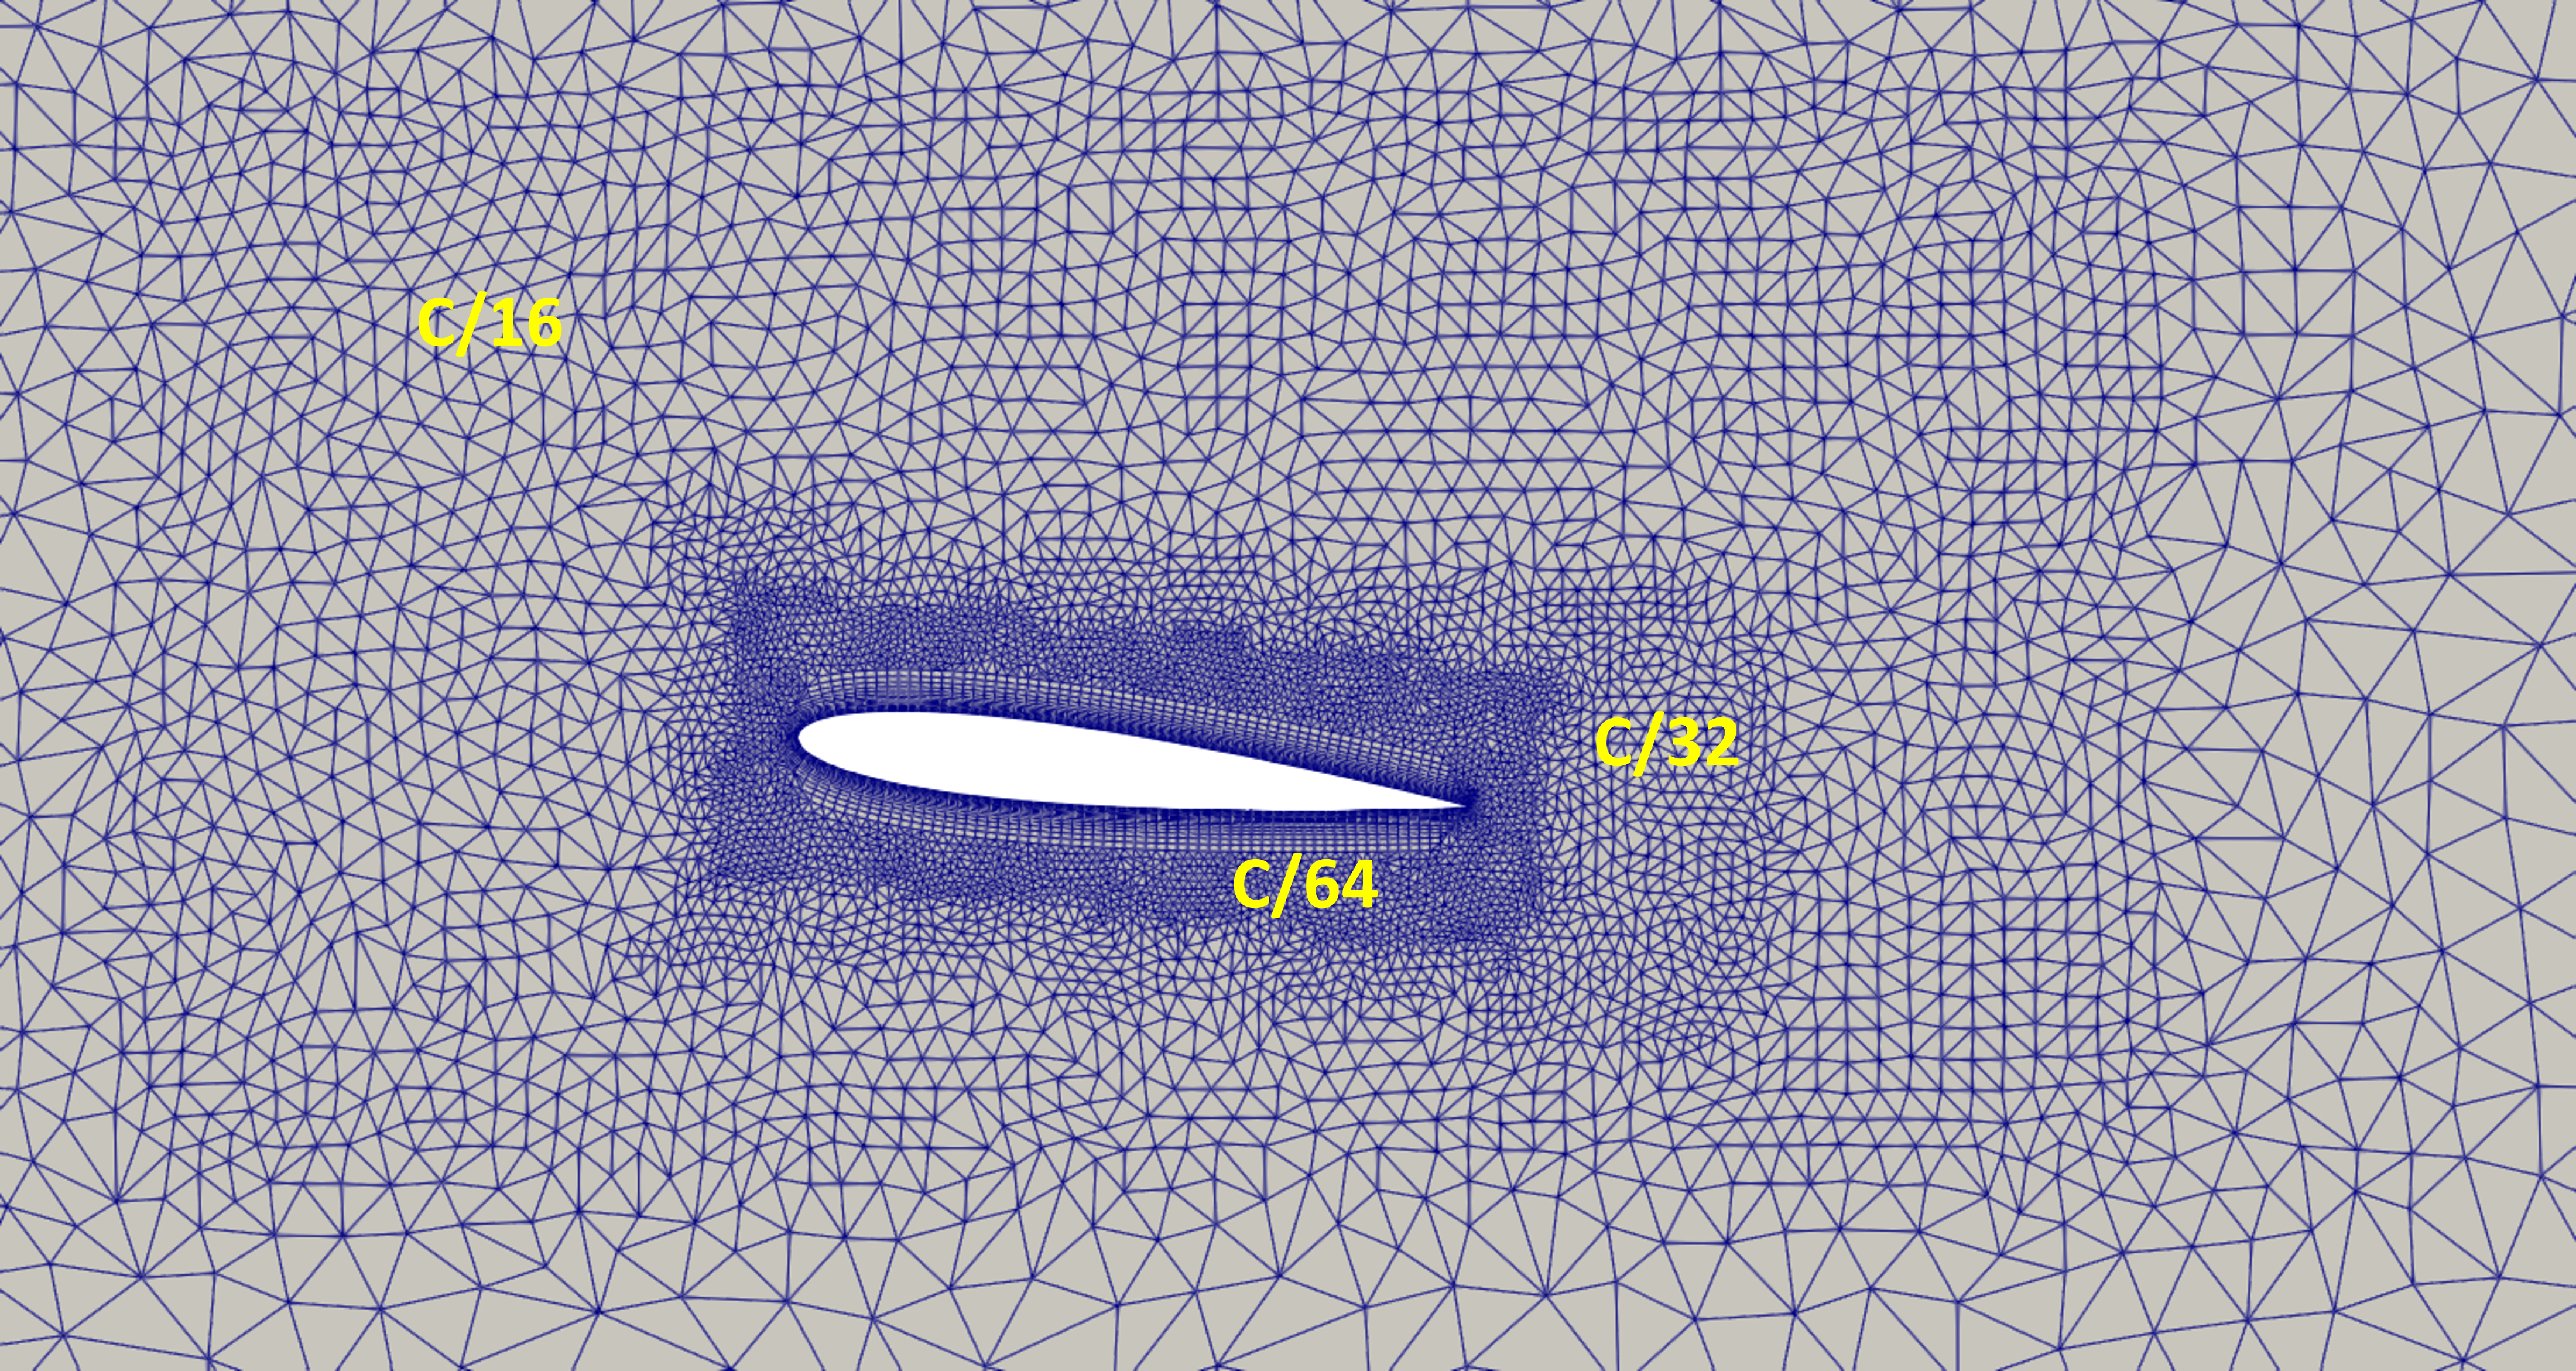
\includegraphics[width=1\textwidth]{figures/adapt_strat/M0_mesh.png}
\caption{M0\_nz25 mesh}
\label{fig:M0_mesh}
\end{subfigure}
\begin{subfigure}[b]{0.475\textwidth}
\centering
\includegraphics[width=1\textwidth]{figures/adapt_strat/M0_error.png}
\caption{M0\_nz25 error field}
\label{fig:M0_err_plot}
\end{subfigure}
\begin{subfigure}[b]{0.475\textwidth}
\centering
\includegraphics[width=1\textwidth]{figures/adapt_strat/Mza1_mesh.png}
\caption{Mza1\_nz50 mesh}
\label{fig:Mza1_mesh}
\end{subfigure}
\begin{subfigure}[b]{0.475\textwidth}
\centering
\includegraphics[width=1\textwidth]{figures/adapt_strat/Mza1_error.png}
\caption{Mza1\_nz50 error field}
\label{fig:Mza1_err_plot}
\end{subfigure}
%\begin{subfigure}[b]{0.475\textwidth}
%\centering
%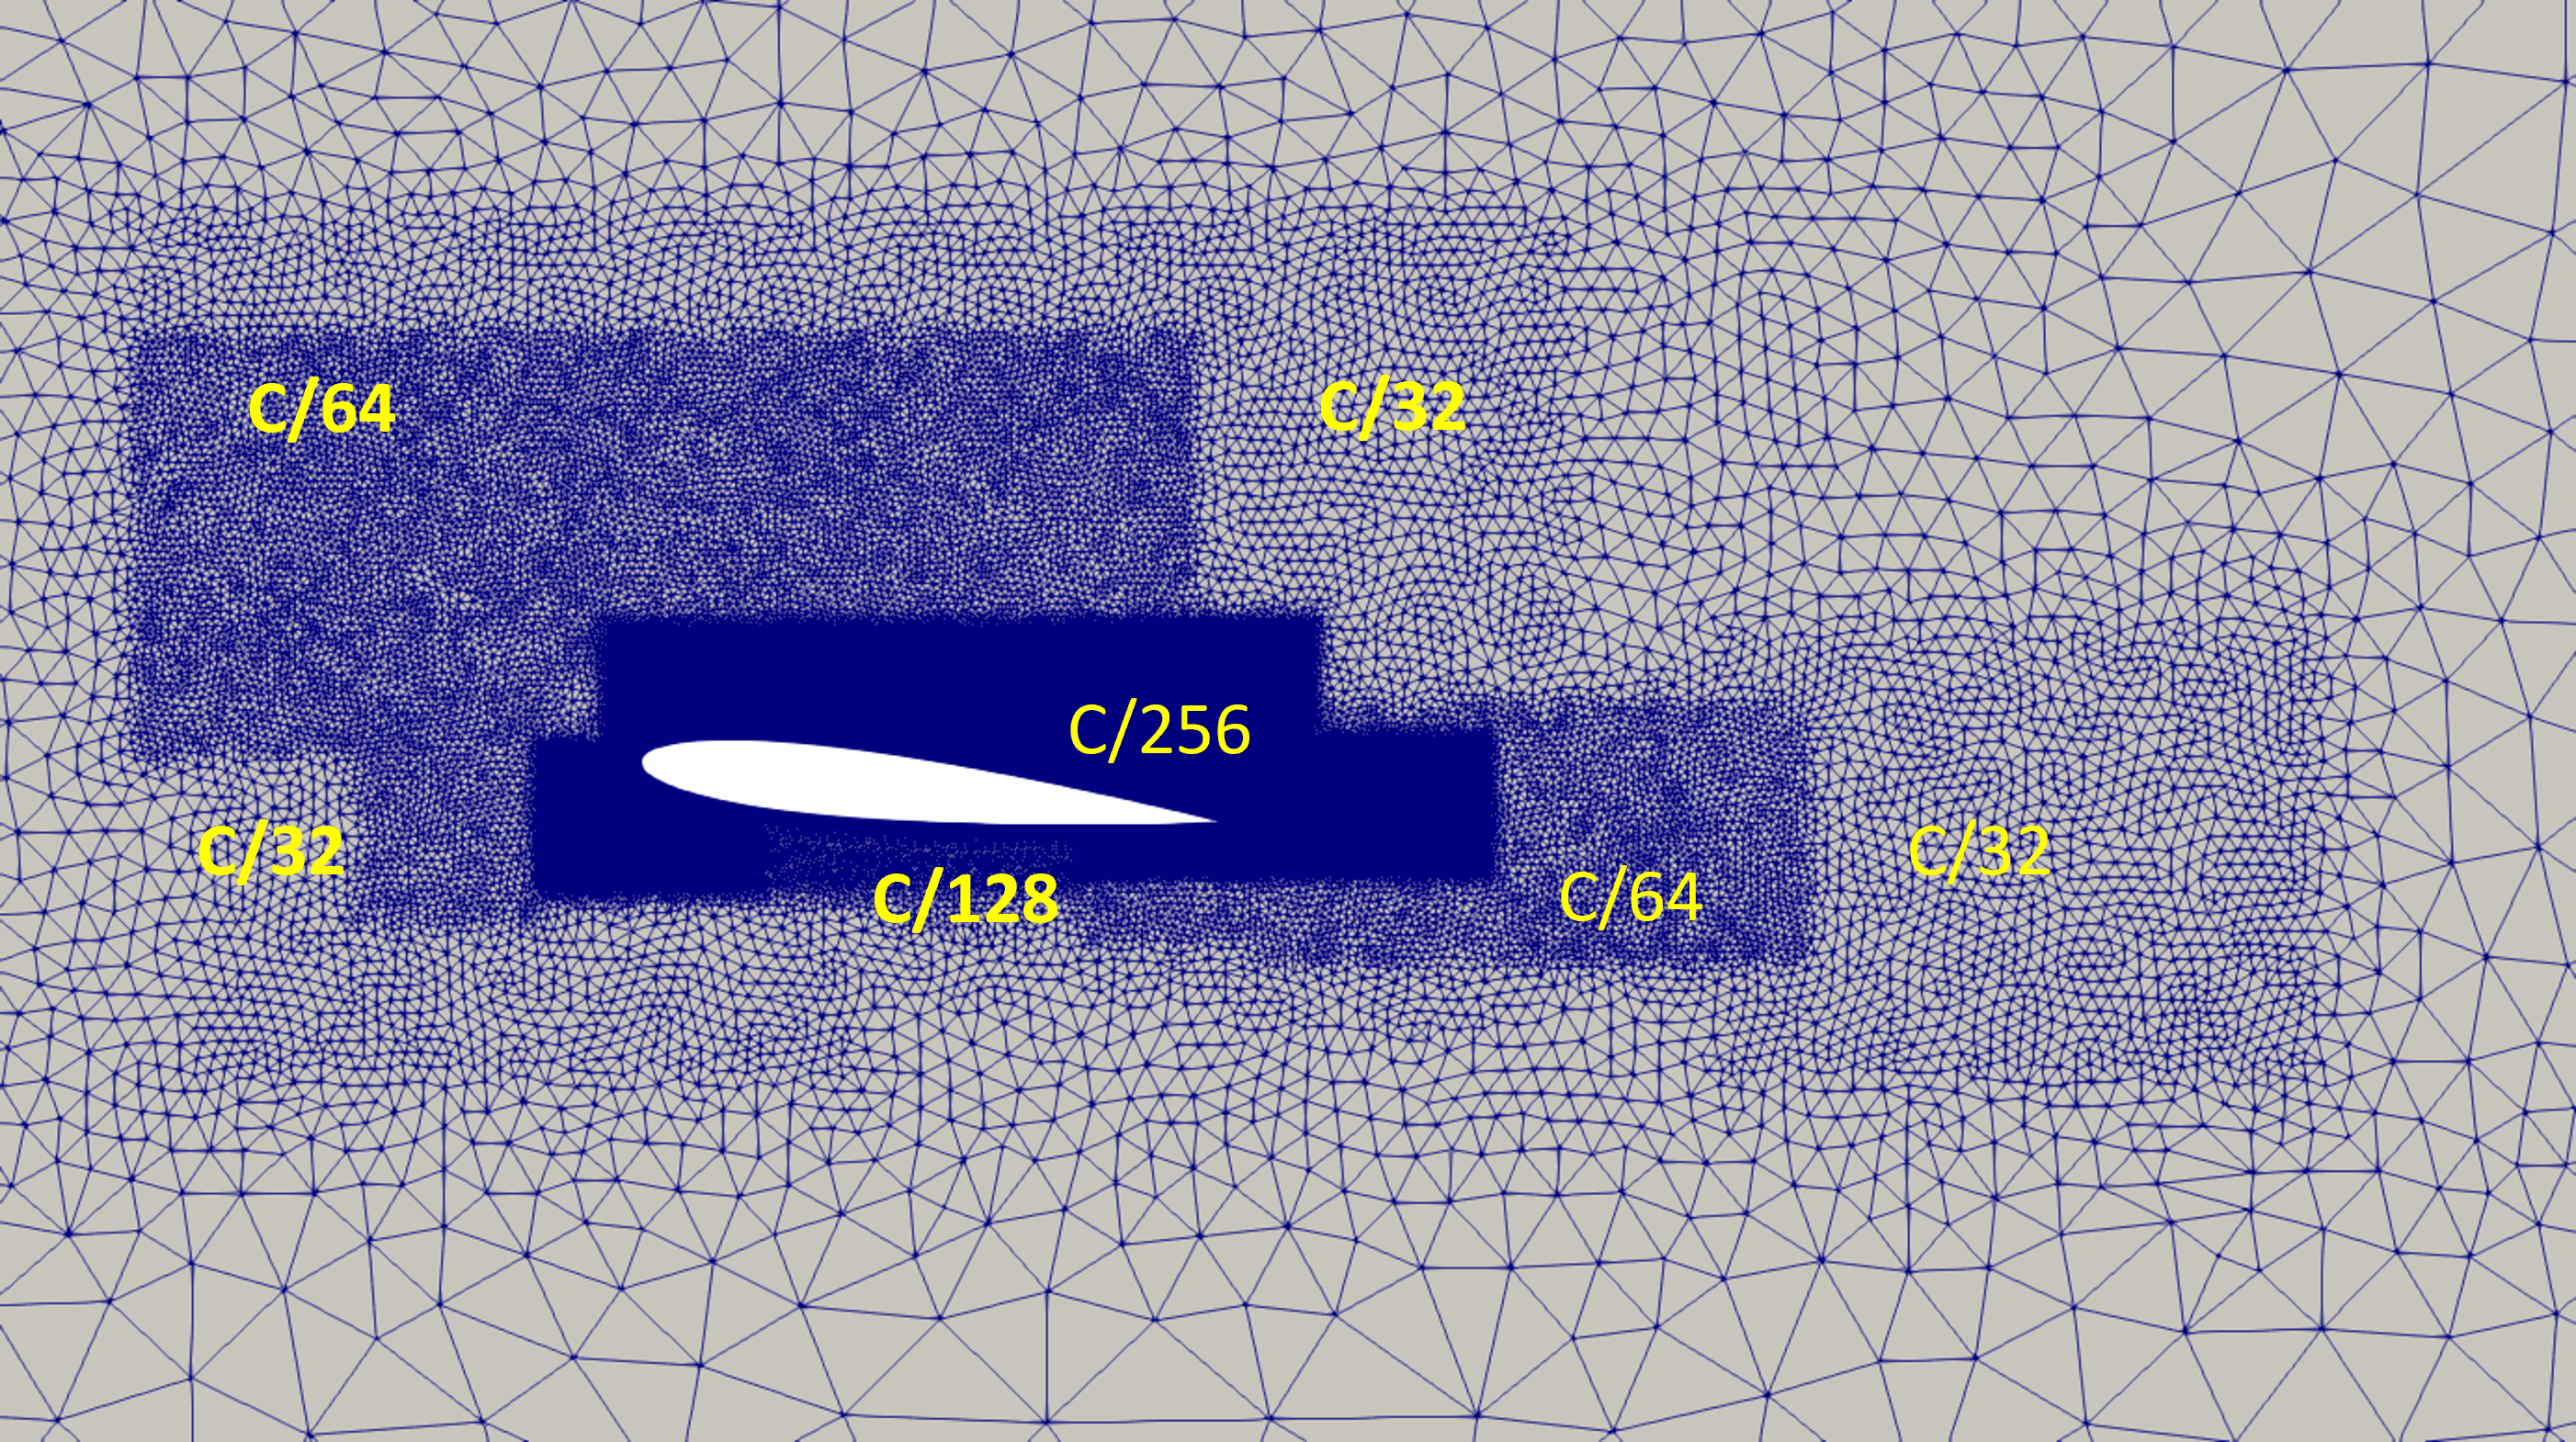
\includegraphics[width=1\textwidth]{figures/adapt_strat/Mza2_mesh.png}
%\caption{Mz\_a2 mesh}
%\label{fig:Mza2_mesh}
%\end{subfigure}
%\begin{subfigure}[b]{0.475\textwidth}
%\centering
%\includegraphics[width=1\textwidth]{figures/adapt_strat/Mza2_error_plot.png}
%\caption{Mz\_a2 error field}
%\label{fig:Mza2_err_plot}
%\end{subfigure}
\caption{Meshes and estimated error fields for zonal-based strategy}
\end{figure}



\subsection{Nodal Size Field-based Adaptation}
In this adaptive strategy, the VMS-based error is calculated on the initial mesh. Based on the estimated error, a nodal size field is calculated using the Equation \eqref{eq:diez}, see Section \ref{sec:sf_adapt}.

% \begin{equation}
% \frac{e_k}{\tilde{e}_k} = \left(\frac{h_{old}}{h_{new}}\right)^{m+N/2} 
% \label{eq:diez}
% \end{equation}

%Here, $e_k$ is the measured local error (in the $\HOne$-seminorm) at an element $k$, $\tilde{e}_k$ is the target error for an element specified by the user, $m$ is the polynomial order of the approximation space (i.e., $m=1$ for the linear finite elements used currently) , and $N$ is the number of spatial dimensions. $h_{old}$ is current size of the element, and $h_{new}$ is the desired new mesh size.
%This new mesh size at the element level is assembled at the node/vertex level to perform mesh adaptation.

\begin{figure}[H]
\centering
\begin{subfigure}[b]{0.475\textwidth}
\centering
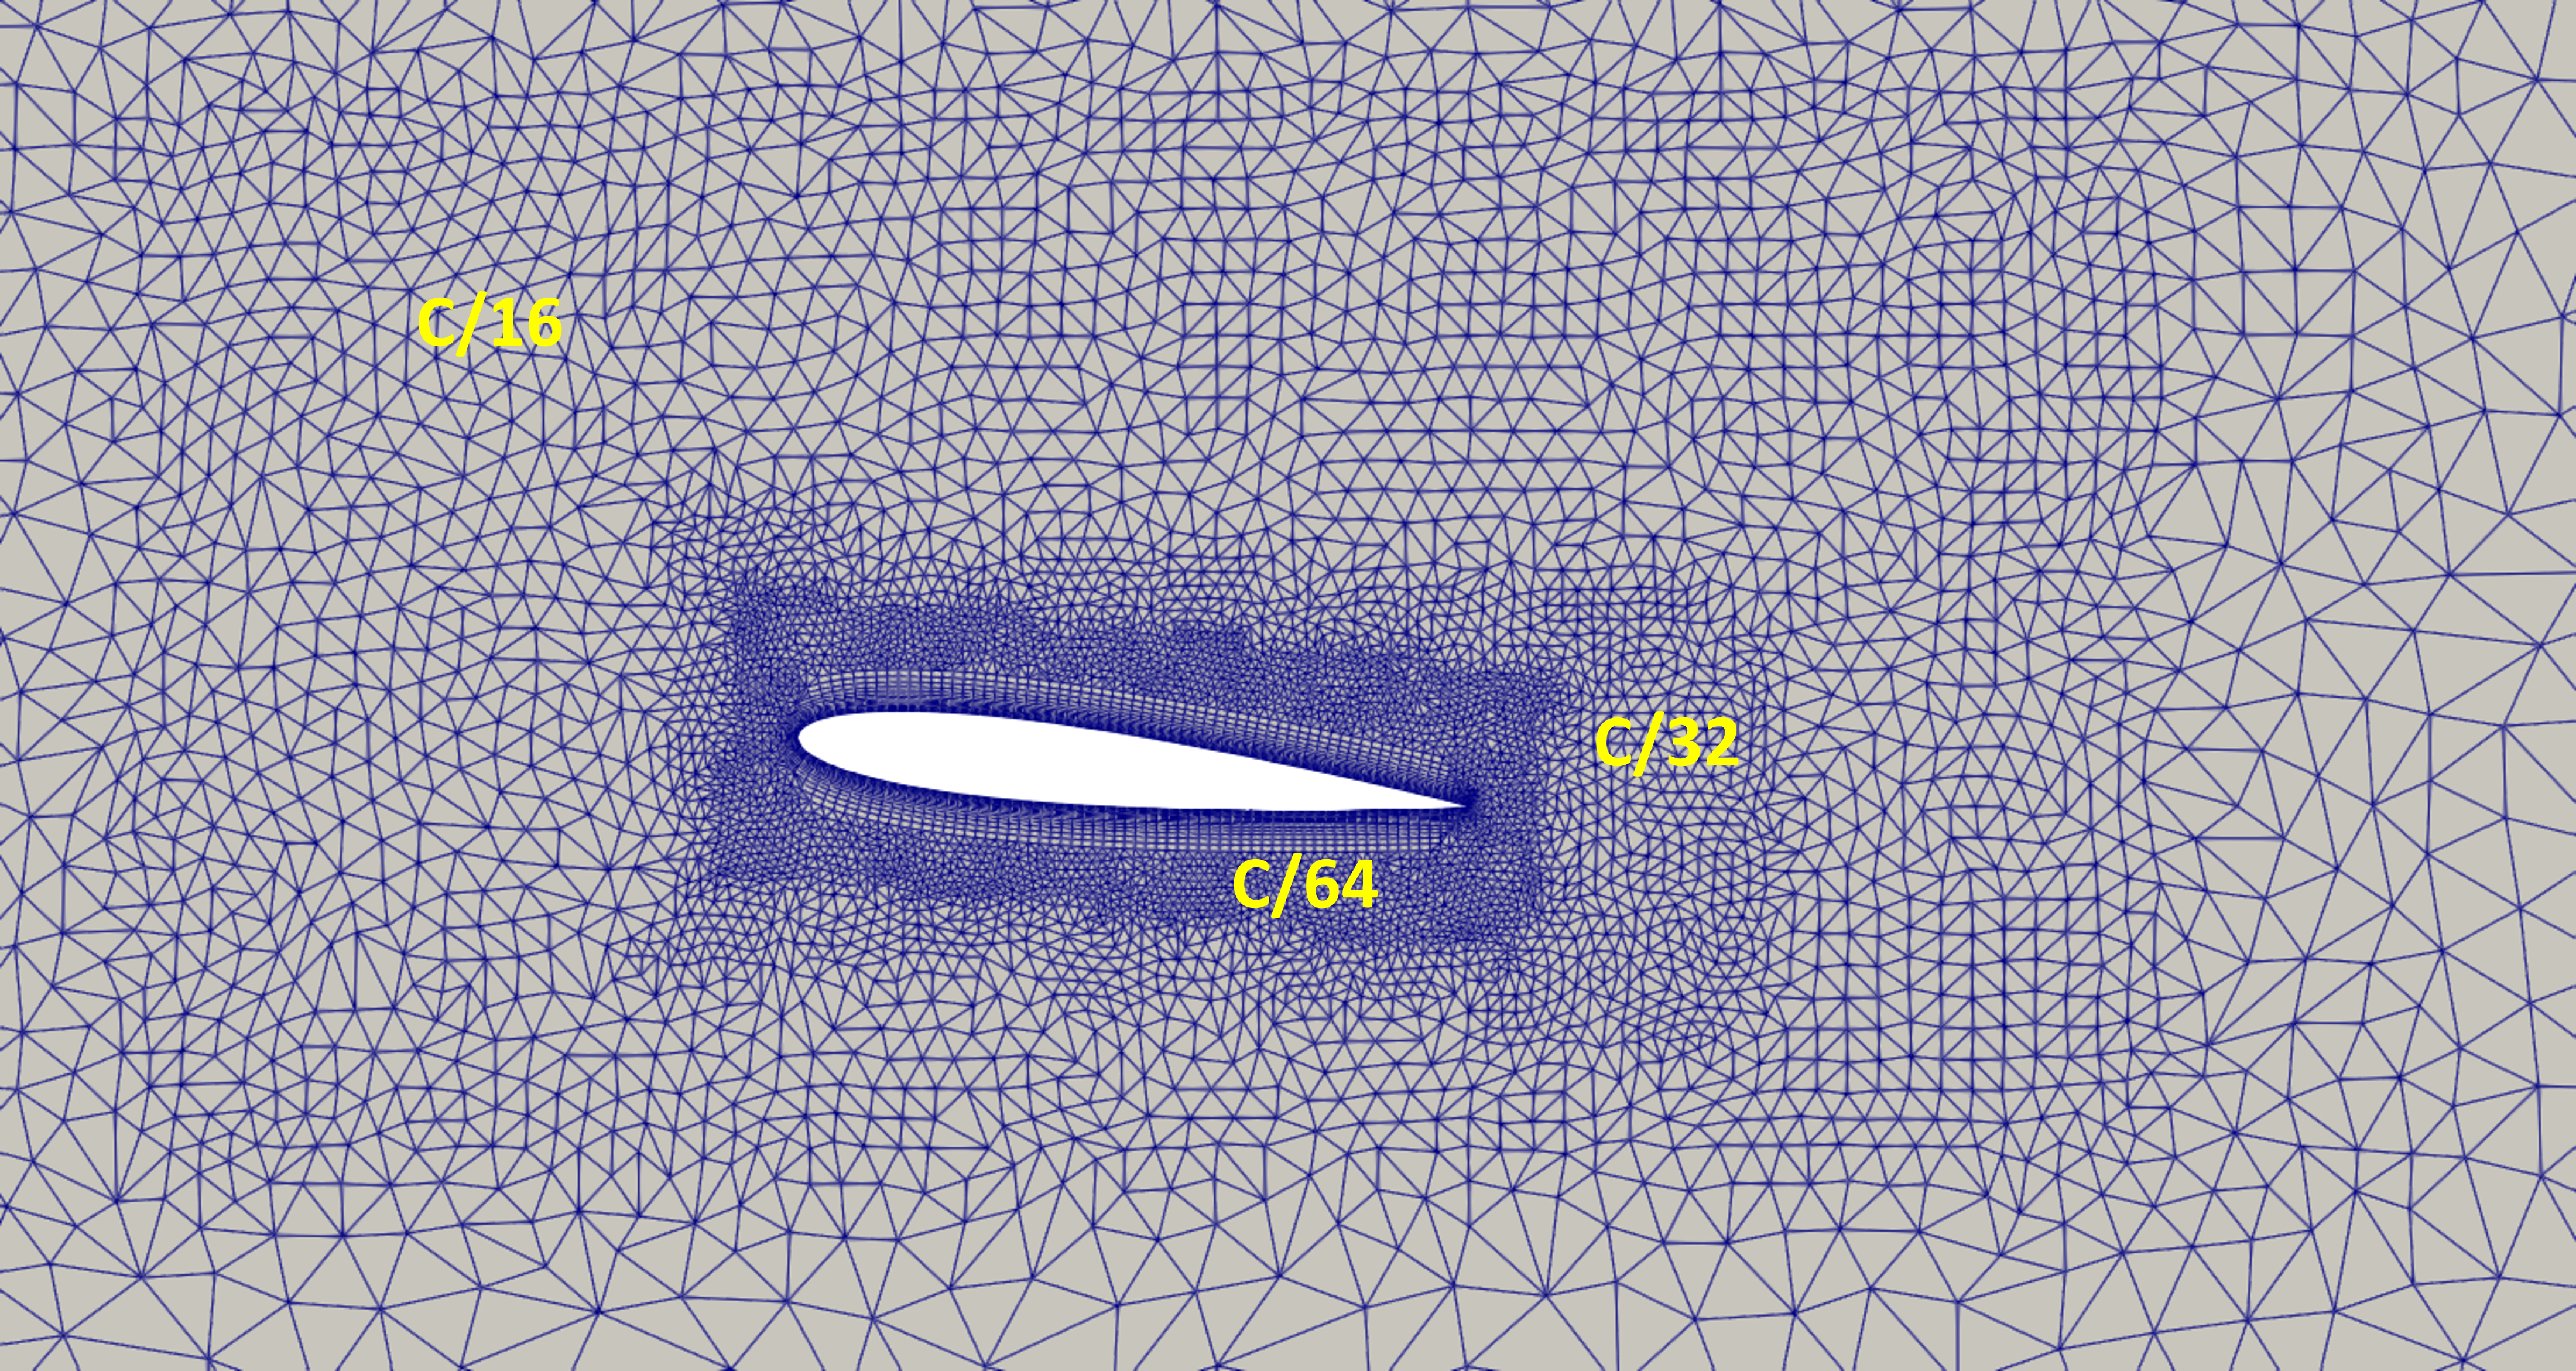
\includegraphics[width=1\textwidth]{figures/adapt_strat/M0_mesh.png}
\caption{M0\_nz25 mesh}
\label{fig:M0_mesh_sa}
\end{subfigure}
\begin{subfigure}[b]{0.475\textwidth}
\centering
\includegraphics[width=1\textwidth]{figures/adapt_strat/M0_error.png}
\caption{M0\_nz25 error field}
\label{fig:M0_err_plot_sa}
\end{subfigure}
\begin{subfigure}[b]{0.475\textwidth}
\centering
\includegraphics[width=1\textwidth]{figures/adapt_strat/Msa1_mesh.png}
\caption{Msa1\_nz50 mesh}
\label{fig:h_adapt1_mesh}
\end{subfigure}
\begin{subfigure}[b]{0.475\textwidth}
\centering
\includegraphics[width=1\textwidth]{figures/adapt_strat/Msa1_error.png}
\caption{Msa1\_nz50 error field}
\label{fig:h_adapt1_error_plot}
\end{subfigure}

\caption{Meshes and estimated error fields for size-based strategy}
\end{figure}

As before, M0\_nz25 is used as the initial mesh (Figure \ref{fig:M0_mesh}) and the corresponding error estimated on M0\_nz25 mesh (Figure \ref{fig:M0_err_plot}) is used to calculate nodal size field (i.e., $h_{new}$ at every mesh node/vertex). The mesh adaptation is limited or controlled to have a maximum refinement and maximum coarsening by a factor of 2 to avoid excessive refinement or coarsening in any local region. The number of extruded layers in the spanwise direction are doubled to 50. The adapted mesh obtained using this strategy is shown in Figure \ref{fig:h_adapt1_mesh}. It is referred to as the Msa1\_nz50 mesh (where sa is short for size-based adaptation and 1 in sa1 denotes the first iteration of mesh adaptation). Note that in terms of mesh resolution, this adapted mesh, Msa1\_nz50, compares well against the Mza1\_nz50 mesh obtained from the zonal-based strategy. Msa1\_nz25 mesh consists of 2,859,450 elements, which is comparable to 2,874,300 elements for the Mza1\_n50 mesh. The major differences between the two meshes is that Mza1\_nz50 maintains the same mesh size in various zones, whereas mesh size varies locally (even within a zone) in Msa1\_nz50.
The corresponding estimated error for this mesh is shown in Figure \ref{fig:h_adapt1_error_plot}. M0\_nz0 mesh and error field are shown again to compare against Msa1\_nz50. Comparing the estimated error between the Msa1\_nz50 and Mza1\_nz50 meshes, higher error values are observed in the LEV regions as well as in the wake of the airfoil. Overall, the estimated error on the Msa1\_nz50 mesh is higher as compared to that on the Mza1\_nz50 mesh. A more detailed comparison of different adaptive strategies/adapted meshes is provided in Section \ref{sec:results_adapt}.


\subsection{Feature-based Refinement}
In this strategy, mesh refinement is applied around the dominant flow features of interest.
In the current surging airfoil case, LEV is the dominant flow feature. 
Using vortex detection and tracking (see Section \ref{sec:LEV_detect_track}), LEV evolution (path and size) is determined using an initial mesh (M0\_nz25 in this case). 
Based on this a refinement zone is added around the path of the LEV.
In such a feature-based refinement, VMS-based estimated error is used to set the mesh size in the refinement zone(s) around the dominant feature(s). 
In addition, estimated error is also used to refine the mesh around the airfoil (e.g., in a similar fashion as the error-based zonal refinement discussed earlier). 
This is done to accurately resolve the flow near the airfoil including the boundary layer region that plays a direct role in the formation of LEV.

In summary, the mesh around the LEV path is refined by a factor of 2. In addition, the boundary layer mesh is refined by a factor of 2 in the streamwise direction, and again, the number of layers in the spanwise direction are doubled as compared to M0\_nz25.
The resulting mesh resolution on the surface of the airfoil in the streamwise and spanwise directions is below 40 and 25 in wall units, respectively, i.e., same as the previous cases.
This adapted mesh is referred to as the Mfa1\_nz50 mesh (where fa is short for feature-based adaptation and 1 in fa1 denotes the first iteration of mesh adaptation). 
This mesh is shown in Figure \ref{fig:FB_mesh} and the estimated error on it is shown in Figure \ref{fig:FB_error_plot}.
M0\_nz0 mesh and error field are shown again to compare against Mfa1\_nz50.
Mfa1\_nz50 contains 2,777,750 elements, which is comparable to both Mza1\_nz50 and Msa1\_nz50 meshes.

Error values are similar to those obtained on the Mza1\_nz50 mesh, i.e., near the airfoil surface, in the LEV path, and in the wake, since mesh resolution in crucial regions is similar between the Mfa1\_nz50 and Mza1\_nz50 meshes, while estimated error is higher on the Msa1\_nz50 mesh.
%Error values are lower as compared to Msa1\_nz50, since a uniform mesh size is maintained, as opposed to Msa1\_nz50, where the mesh size is patchy.
A more detailed comparison of different adaptive strategies/adapted meshes is provided in Section \ref{sec:results_adapt}.

\begin{figure}[H]
\centering
\begin{subfigure}[b]{0.475\textwidth}
\centering
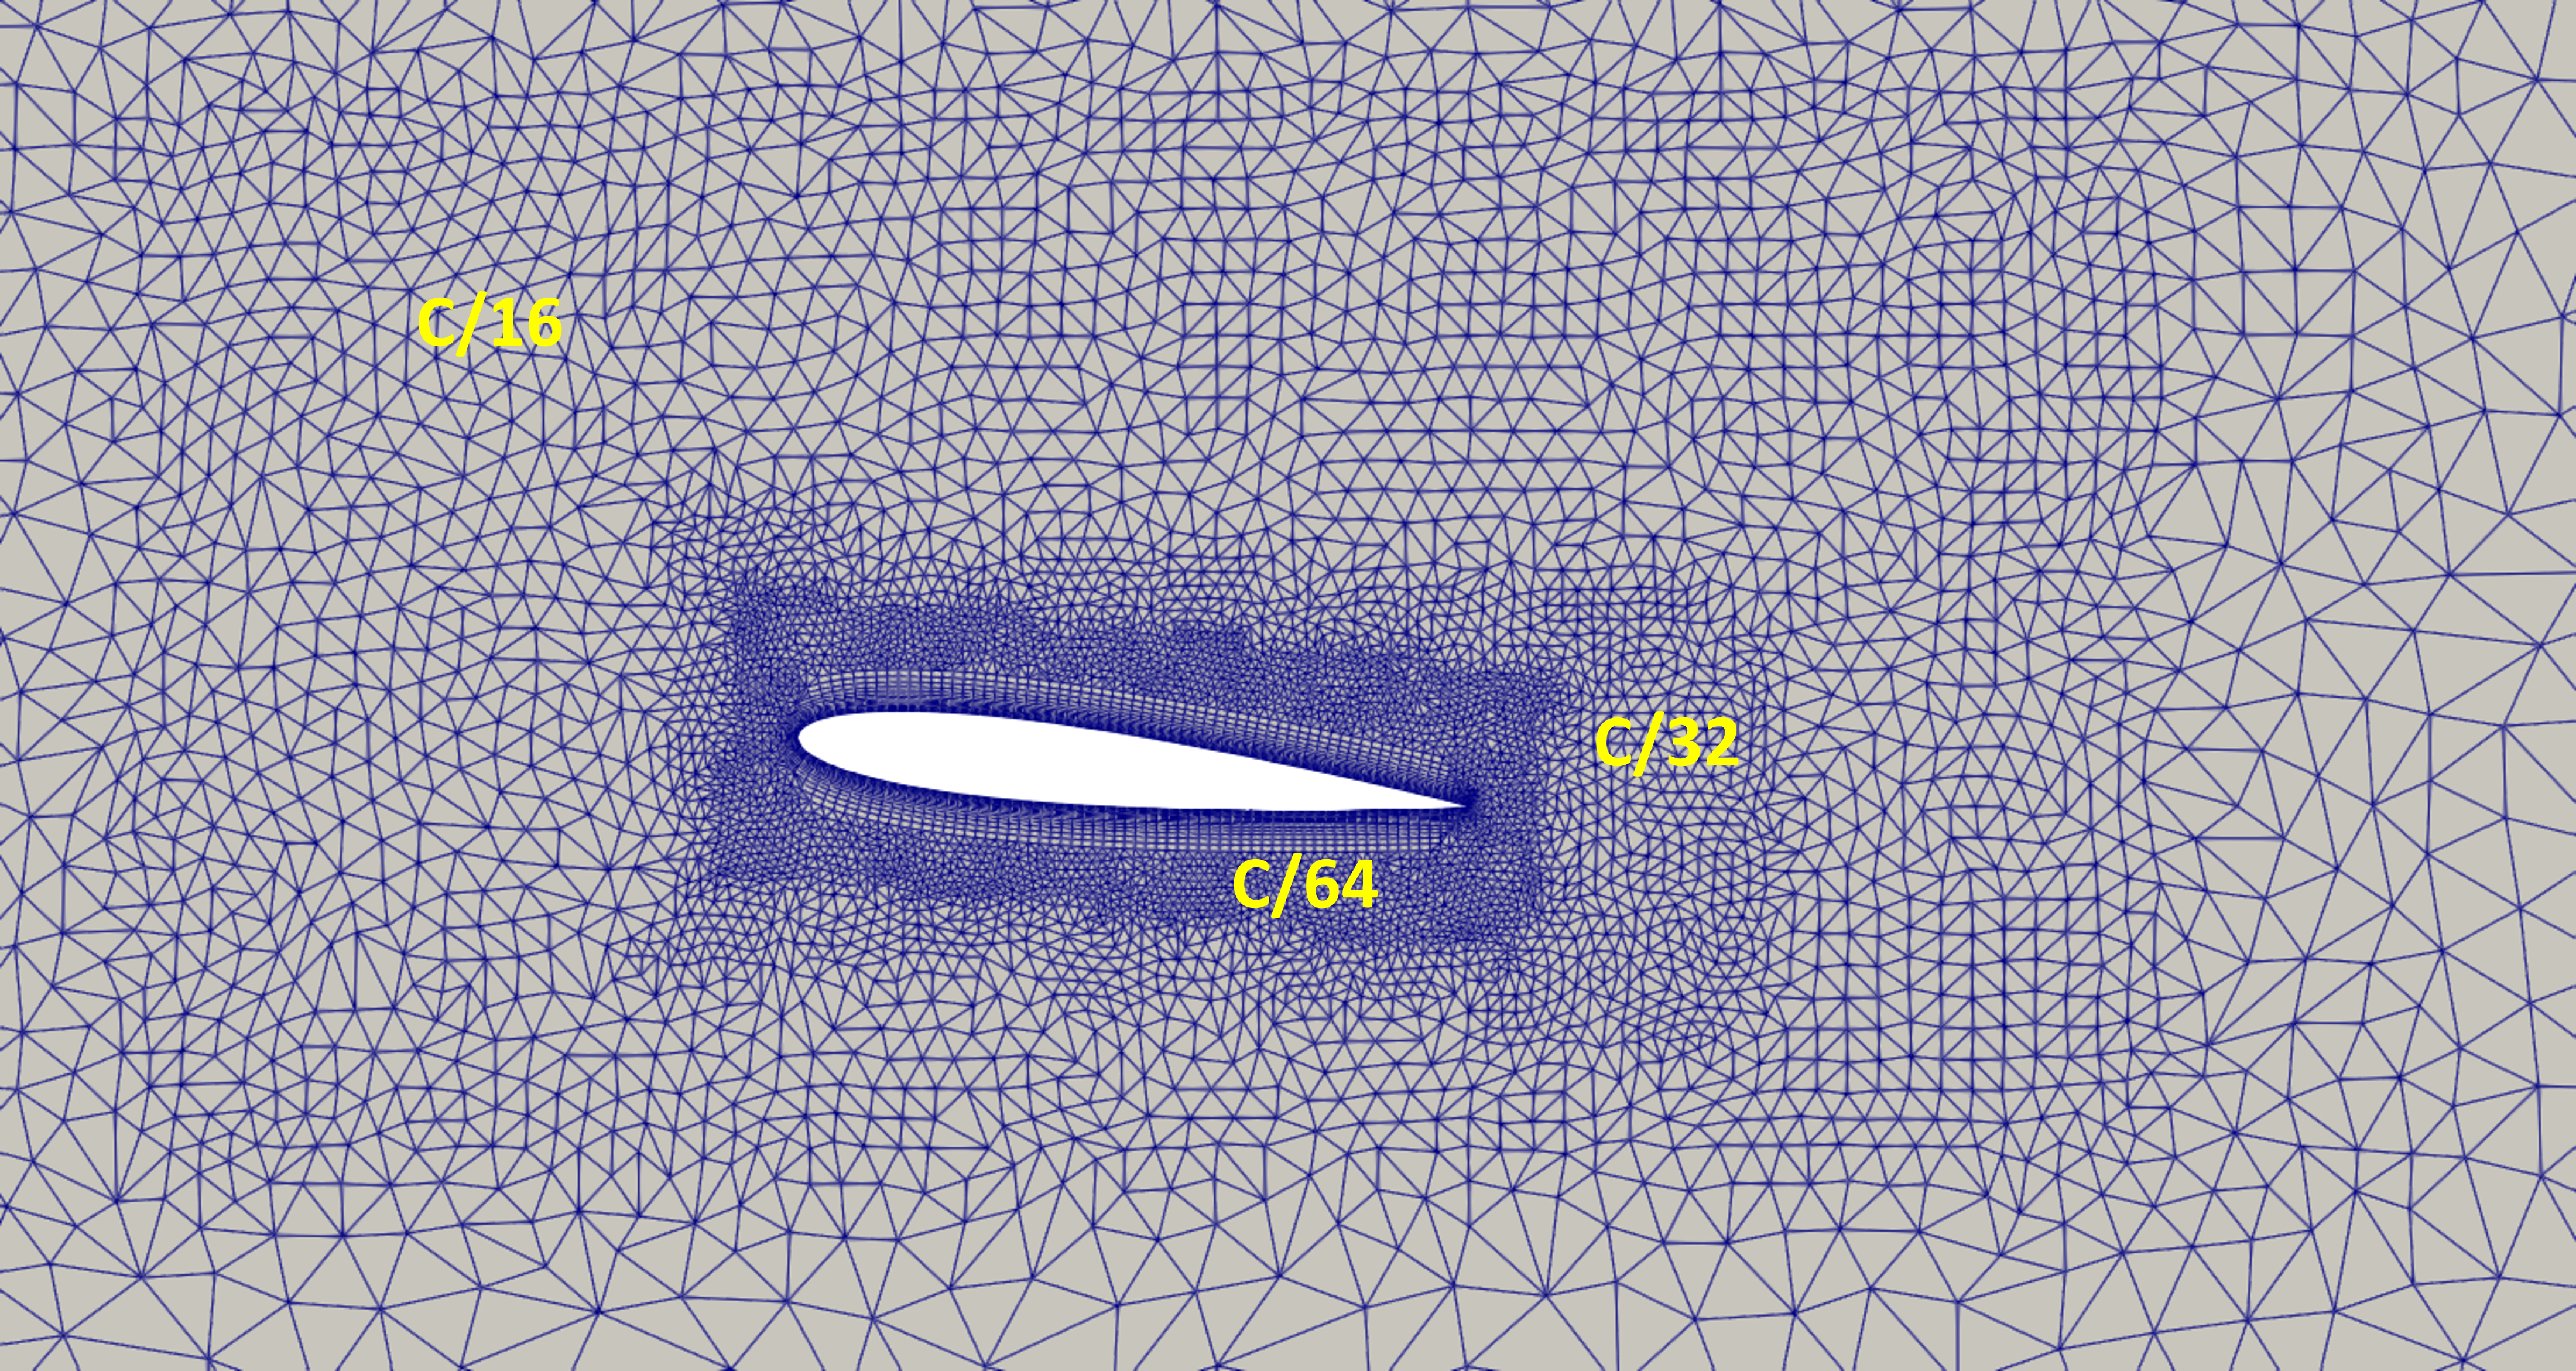
\includegraphics[width=1\textwidth]{figures/adapt_strat/M0_mesh.png}
\caption{M0\_nz25 mesh}
\label{fig:M0_mesh_fa}
\end{subfigure}
\begin{subfigure}[b]{0.475\textwidth}
\centering
\includegraphics[width=1\textwidth]{figures/adapt_strat/M0_error.png}
\caption{M0\_nz25 error field}
\label{fig:M0_err_plot_fa}
\end{subfigure}
\begin{subfigure}[b]{0.475\textwidth}
\centering
\includegraphics[width=1\textwidth]{figures/adapt_strat/Mfa1_mesh.png}
\caption{Mfa1\_nz50 mesh}
\label{fig:FB_mesh}
\end{subfigure}
\begin{subfigure}[b]{0.475\textwidth}
\centering
\includegraphics[width=1\textwidth]{figures/adapt_strat/Mfa1_error.png}
\caption{Mfa1\_nz50 error field}
\label{fig:FB_error_plot}
\end{subfigure}

\caption{Meshes and estimated error fields for feature-based strategy}
\end{figure}
\label{sec:feature_based_strat}


\subsection{Results and Discussion}
In this section, we compare results of different adapted meshes obtained from three adaptive strategies mentioned above. 
We compare different quantities of interest. 
A comparison of force response in the form of normalized lift and drag forces is shown in Figures \ref{fig:lift_plot} and \ref{fig:drag_plot}, respectively. The normalized lift and drag matches up well for all the adapted meshes.

A comparison of spanwise vorticity for the different adapted meshes is shown in Figures \ref{fig:vorticity_195}, \ref{fig:vorticity_210} and \ref{fig:vorticity_270}, for 3 phases of $\psi=210^\circ$, $\psi=225^\circ$ and $\psi=270^\circ$, respectively.
For $\psi=195^\circ$, as the airfoil is in the retreating phase, boundary layer roll-up towards the geometric leading edge is observed over the airfoil surface.
For the meshes based on zonal refinement, as we go from M0\_nz25 to Mza1\_nz50, the separation over the airfoil is well resolved, and finer scales or flow structures are visible on the adapted mesh.
Comparing Mza1\_nz50, Msa1\_nz50, and Mfa1\_nz50 meshes, we can see that the Msa1\_nz50 mesh (sizefield-based adapted mesh) does not capture the finer scales/structures as compared to the Mza1\_nz50 mesh, both over the airfoil surface and in the wake of the airfoil, i.e., flow structures are more diffused in the case of Msa1\_nz50.
On the other hand, the Mfa1\_nz50 mesh captures them well.

\begin{figure}[H]
\centering

\begin{subfigure}[b]{0.7\textwidth}
\centering
\includegraphics[width=1\textwidth]{figures/Results/Lift_adapt_strat.png}
\caption{Normalized lift}
\label{fig:lift_plot}
\end{subfigure}
\begin{subfigure}[b]{0.7\textwidth}
\centering
\includegraphics[width=1\textwidth]{figures/Results/Drag_adapt_strat.png}
\caption{Normalized drag}
\label{fig:drag_plot}
\end{subfigure}

\label{fig:force_response_adapt}
\caption{Normalized forces for different adaptive strategies/adapted meshes}
\end{figure}

%Next, we look at the location of the LEV core for different meshes in Figure \ref{fig:LEV_location}. Some differences in the LEV location for various phases are observed. LEV location for Ma1, FB, and hadapt meshes is similar in the beginning phases. Ma1 starts to deviate from FB and hadapt in the later phases. LEV location for FB and hadapt meshes start to match with Ma2 in the later phases, whereas M0 LEV location fluctuates around the other meshes. This however is still not conclusive as to which mesh performs better and a more quantitative study is needed.


%%\begin{figure}[H]
%\centering
%\includegraphics[width=0.7\textwidth]{figures/Results/LEV_location.png}
%\caption{LEV location for different meshes}
%\label{fig:LEV_location}
%\end{figure}
%%


For $\psi=210^\circ$, formation of LEV begins to take place, as we start to see the roll-up of separated shear layer near the geometric leading edge. 
At this phase, the differences in the structures resolved by the different meshes become more clear.
Similar to $\psi=195^\circ$, the Msa1\_nz50 mesh shows a relatively poor resolution of the finer flow structures as compared to the Mza1\_nz50 and Mfa1\_nz50 meshes.

For $\psi=270^\circ$, differences can be seen in the separated shear layer at the geometric leading edge of the airfoil, and the resolution of the LEV, among different adapted meshes.
These are resolved better on the Mfa1\_nz50 and Mza1\_nz50 meshes. 
Recall that Mfa1\_nz50 is obtained using feature-based mesh refinement designed to capture the LEV accurately, and has the same mesh resolution as Mza1\_nz50 along the path of the LEV. 
%Once again, shear layer is not well resolved for Msa1\_nz50 as compared to other refined/adapted meshes.

The relatively poor resolution of flow, with more diffused flow structures, observed for Msa1\_nz50 can be attributed to the variation in mesh sizes (even by a factor of 1.5 or 2) in crucial regions of interest, i.e., the mesh size is not uniform or even quasi-uniform in particular zones. In particular, this seem to have an adverse effect in regions with turbulence.

\begin{figure}[H]
\centering
\begin{subfigure}[b]{0.475\textwidth}
\centering
\includegraphics[width=1\textwidth]{figures/adapt_strat/vorticity_plots/M0/phase_195.png}
\caption{M0\_nz25 mesh, $\psi$ = $195^\circ$}
\label{fig:M0_psi195}
\end{subfigure}
\begin{subfigure}[b]{0.475\textwidth}
\centering
\includegraphics[width=1\textwidth]{figures/adapt_strat/vorticity_plots/Mza1_50/phase_195.png}
\caption{Mza1\_nz50 mesh, $\psi$ = $195^\circ$}
\label{fig:Ma1_psi195}
\end{subfigure}
%\begin{subfigure}[b]{0.475\textwidth}
%\centering
%\includegraphics[width=1.25\textwidth]{figures/vorticity_plots/Mza2/ph_195.png}
%\caption{Mz\_a2 mesh, $\psi$ = $195^\circ$}
%\label{fig:Ma2_psi195}
%\end{subfigure}
\begin{subfigure}[b]{0.475\textwidth}
\centering
\includegraphics[width=1\textwidth]{figures/adapt_strat/vorticity_plots/Msa1_50/phase_195.png}
\caption{Msa1\_nz50 mesh, $\psi$ = $195^\circ$}
\label{fig:hadapt_psi195}
\end{subfigure}
\begin{subfigure}[b]{0.475\textwidth}
\centering
\includegraphics[width=1\textwidth]{figures/adapt_strat/vorticity_plots/Mfa1_50/phase_195.png}
\caption{Mfa1\_nz50 mesh, $\psi$ = $195^\circ$}
\label{fig:FB_psi195}
\end{subfigure}
\caption{Spanwise vorticity comparison at $\psi$ = $195^\circ$ for different adaptive strategies/adapted meshes}
\label{fig:vorticity_195}
\end{figure}



\begin{figure}[H]
\centering
\begin{subfigure}[b]{0.475\textwidth}
\centering
\includegraphics[width=1\textwidth]{figures/adapt_strat/vorticity_plots/M0/phase_210.png}
\caption{M0\_nz25 mesh, $\psi$ = $210^\circ$}
\label{fig:M0_psi210}
\end{subfigure}
\begin{subfigure}[b]{0.475\textwidth}
\centering
\includegraphics[width=1\textwidth]{figures/adapt_strat/vorticity_plots/Mza1_50/phase_210.png}
\caption{Mza1\_nz50 mesh, $\psi$ = $210^\circ$}
\label{fig:Mza1_psi210}
\end{subfigure}
%\begin{subfigure}[b]{0.475\textwidth}
%\centering
%\includegraphics[width=1.25\textwidth]{figures/vorticity_plots/Mza2/ph_210.png}
%\caption{Mz\_a2 mesh, $\psi$ = $210^\circ$}
%\label{fig:Ma2_psi210}
%\end{subfigure}
\begin{subfigure}[b]{0.475\textwidth}
\centering
\includegraphics[width=1\textwidth]{figures/adapt_strat/vorticity_plots/Msa1_50/phase_210.png}
\caption{Msa1\_nz50 mesh, $\psi$ = $210^\circ$}
\label{fig:hadapt_psi210}
\end{subfigure}
\begin{subfigure}[b]{0.475\textwidth}
\centering
\includegraphics[width=1\textwidth]{figures/adapt_strat/vorticity_plots/Mfa1_50/phase_210.png}
\caption{Mfa1\_nz50 mesh, $\psi$ = $210^\circ$}
\label{fig:FB_psi210}
\end{subfigure}
\caption{Spanwise vorticity comparison at $\psi$ = $210^\circ$ for different adaptive strategies/adapted meshes}
\label{fig:vorticity_210}
\end{figure}



%%VORTICITY PLOT
\begin{figure}[H]
\centering

\begin{subfigure}[b]{0.475\textwidth}
\centering
\includegraphics[width=1\textwidth]{figures/adapt_strat/vorticity_plots/M0/phase_270.png}
\caption{M0\_nz25 mesh, $\psi$ = $270^\circ$}
\label{fig:M0_psi270}
\end{subfigure}
\begin{subfigure}[b]{0.475\textwidth}
\centering
\includegraphics[width=1\textwidth]{figures/adapt_strat/vorticity_plots/Mza1_50/phase_270.png}
\caption{Mza1\_nz50 mesh, $\psi$ = $270^\circ$}
\label{fig:Ma1_psi270}
\end{subfigure}
%\begin{subfigure}[b]{0.475\textwidth}
%\centering
%\includegraphics[width=1.25\textwidth]{figures/vorticity_plots/Mza2/ph_270.png}
%\caption{Mz\_a2 mesh, $\psi$ = $270^\circ$}
%\label{fig:Ma2_psi270}
%\end{subfigure}
\begin{subfigure}[b]{0.475\textwidth}
\centering
\includegraphics[width=1\textwidth]{figures/adapt_strat/vorticity_plots/Msa1_50/phase_270.png}
\caption{Msa1\_nz50 mesh, $\psi$ = $270^\circ$}
\label{fig:hadapt_psi270}
\end{subfigure}
\begin{subfigure}[b]{0.475\textwidth}
\centering
\includegraphics[width=1\textwidth]{figures/adapt_strat/vorticity_plots/Mfa1_50/phase_270.png}
\caption{Mfa1\_nz50 mesh, $\psi$ = $270^\circ$}
\label{fig:FB_psi270}
\end{subfigure}
\caption{Spanwise vorticity comparison at $\psi$ = $270^\circ$ for different adaptive strategies/adapted meshes}
\label{fig:vorticity_270}
\end{figure}

Figures \ref{fig:Mza1_zoomed}, \ref{fig:Msa1_zoomed} and \ref{fig:Mfa1_zoomed} show a zoomed-in view of the mesh, spanwise vorticity at $\psi=210^\circ$, and the element-level/local error (maximum over multiple phases and over the spanwise direction). This is done for Mza1\_nz50, Msa1\_nz50, and Mfa1\_nz50 meshes.
The different meshes in these figures show that a quasi-uniform mesh size is maintained in specified zones for both Mza1\_nz50 and Mfa1\_nz50, while the Msa1\_nz50 mesh is patchy, i.e., a uniform mesh size is not maintained in Msa1\_nz50.
The error field for Msa1\_nz50 is also patchy, as compared to Mza1\_nz50 and Mfa1\_nz50, with elements that have a higher local estimated error in Msa1\_nz50.
This becomes further evident from the vorticity plots, especially in the wake region, where Msa1\_nz50 shows a poor resolution of fine-scale flow structures, as compared to Mza1\_nz50 and Mfa1\_nz50.
Note that the Mza1\_nz50 and Mfa1\_nz50 meshes are very comparable and the zonal refinement encompasses the regions/portions covered by the feature/LEV-based refinement, and thus, they turn out to be equivalent for the current case.

\begin{figure}[H]
	\centering
\begin{subfigure}[b]{0.7\textwidth}
	\centering
	\includegraphics[width=1\textwidth]{figures/adapt_strat/zoomed/Mza1_mesh.png}
	\caption{Mza1\_nz50 mesh}
	\label{fig:Mza1_mesh_zoomed}
\end{subfigure}
\begin{subfigure}[b]{0.7\textwidth}
	\centering
	\includegraphics[width=1\textwidth]{figures/adapt_strat/zoomed/Mza1_error.png}
	\caption{Mza1\_nz50 estimated error}
	\label{fig:Mza1_max_error_zoomed}
\end{subfigure}
\begin{subfigure}[b]{0.7\textwidth}
	\centering
	\includegraphics[width=1\textwidth]{figures/adapt_strat/zoomed/Mza1_ph_210.png}
	\caption{Mza1\_nz50 vorticity at $\psi=210^\circ$}
	\label{fig:Mza1_vorticity_zoomed}
\end{subfigure}
\caption{Zoomed-in view for Mza1\_nz50: mesh, estimated error and vorticity}
\label{fig:Mza1_zoomed}
\end{figure}

\begin{figure}[H]
	\centering
	\begin{subfigure}[b]{0.7\textwidth}
		\centering
		\includegraphics[width=1\textwidth]{figures/adapt_strat/zoomed/Msa1_mesh.png}
		\caption{Msa1\_nz50 mesh}
		\label{fig:Msa1_mesh_zoomed}
	\end{subfigure}
	\begin{subfigure}[b]{0.7\textwidth}
		\centering
		\includegraphics[width=1\textwidth]{figures/adapt_strat/zoomed/Msa1_error.png}
		\caption{Msa1\_nz50 estimated error}
		\label{fig:Msa1_max_error_zoomed}
	\end{subfigure}
	\begin{subfigure}[b]{0.7\textwidth}
		\centering
		\includegraphics[width=1\textwidth]{figures/adapt_strat/zoomed/Msa1_ph_210.png}
		\caption{Msa1\_nz50 vorticity at $\psi=210^\circ$}
		\label{fig:Msa1_vorticity_zoomed}
	\end{subfigure}
	\caption{Zoomed-in view for Msa1\_nz50: mesh, estimated error and vorticity}
	\label{fig:Msa1_zoomed}
\end{figure}


\begin{figure}[H]
	\centering
	\begin{subfigure}[b]{0.7\textwidth}
		\centering
		\includegraphics[width=1\textwidth]{figures/adapt_strat/zoomed/Mfa1_mesh.png}
		\caption{Mfa1\_nz50 mesh}
		\label{fig:Mfa1_mesh_zoomed}
	\end{subfigure}
	\begin{subfigure}[b]{0.7\textwidth}
		\centering
		\includegraphics[width=1\textwidth]{figures/adapt_strat/zoomed/Mfa1_error.png}
		\caption{Mfa1\_nz50 estimated error}
		\label{fig:Mfa1_max_error_zoomed}
	\end{subfigure}
	\begin{subfigure}[b]{0.7\textwidth}
		\centering
		\includegraphics[width=1\textwidth]{figures/adapt_strat/zoomed/Mfa1_ph_210.png}
		\caption{Mfa1\_nz50 vorticity at $\psi=210^\circ$}
		\label{fig:Mfa1_vorticity_zoomed}
	\end{subfigure}
	\caption{Zoomed-in view for Mfa1\_nz50: mesh, estimated error and vorticity}
	\label{fig:Mfa1_zoomed}
\end{figure}



For a more quantitative comparison, we focus on pressure coefficient, $C_p$,  at different phases of interest including those around LEV formation. $C_p$ is shown in Figure \ref{fig:Cp_plots} at six phases for all adapted meshes. At $\psi=180^\circ$, we can see that flow has started to separate for all meshes apart from M0\_nz25. For $\psi=195^\circ$, Msa1\_nz50 shows a larger $C_p$ value as compared to the other meshes, with M0\_nz25 showing the lowest $C_p$. For $\psi=210^\circ$, LEV presence is seen for all meshes apart from M0\_nz25 mesh. $\psi=225^\circ$ shows LEV presence and flow separation for all meshes, with some differences in separation location for Msa1\_nz50 as compared to Mza1\_nz50 and Mfa1\_nz50. Note that a different range of $C_p$ is used for each phase to highlight the differences. At
$\psi=270^\circ$ and $\psi=285^\circ$, marginal differences are seen in $C_p$ among different meshes, specifically at the geometric trailing edge where flow separation starts to occur. 

%%Cp plots

\begin{figure}[H]
\centering

\begin{subfigure}[b]{0.475\textwidth}
\centering
\includegraphics[width=1\textwidth]{figures/Results/Cp_plots/Cp_ph_180.png}
\caption{ $C_p$ at $\psi$ = $180^\circ$}
\label{fig:Cp_180}
\end{subfigure}
\begin{subfigure}[b]{0.475\textwidth}
\centering
\includegraphics[width=1\textwidth]{figures/Results/Cp_plots/Cp_ph_195.png}
\caption{ $C_p$ at $\psi$ = $195^\circ$}
\label{fig:Cp_195}
\end{subfigure}
\begin{subfigure}[b]{0.475\textwidth}
\centering
\includegraphics[width=1\textwidth]{figures/Results/Cp_plots/Cp_ph_210.png}
\caption{ $C_p$ at $\psi$ = $210^\circ$}
\label{fig:Cp_210}
\end{subfigure}
\begin{subfigure}[b]{0.475\textwidth}
\centering
\includegraphics[width=1\textwidth]{figures/Results/Cp_plots/Cp_ph_225.png}
\caption{ $C_p$ at $\psi$ = $225^\circ$}
\label{fig:Cp_225}
\end{subfigure}
\begin{subfigure}[b]{0.475\textwidth}
\centering
\includegraphics[width=1\textwidth]{figures/Results/Cp_plots/Cp_ph_270.png}
\caption{ $C_p$ at $\psi$ = $270^\circ$}
\label{fig:Cp_270}
\end{subfigure}
\begin{subfigure}[b]{0.475\textwidth}
\centering
\includegraphics[width=1\textwidth]{figures/Results/Cp_plots/Cp_ph_285.png}
\caption{ $C_p$ at $\psi$ = $285^\circ$}
\label{fig:Cp_285}
\end{subfigure}
\caption{$C_p$ comparison for different meshes. Top surface $C_p$ is denoted by solid lines and bottom surface $C_p$ is denoted by dashed lines}
\label{fig:Cp_plots}
\end{figure}

In summary, mesh refinement/adaptation is necessary to perform accurate LES of complex aerodynamic problems. The above comparison among different adaptive strategies clearly indicates that the zonal-based refinement/adaptation strategy is the most appropriate for the current problem of interest involving surging airfoils. Thus, it is used subsequently to construct a series of adapted meshes and demonstrate mesh convergence.
\label{sec:results_adapt}

\label{adapt_strat}

\include{bibtex_database.bib} % bibliography
\include{rpiapp} % appendix


 
\end{document}
